\lecture{Modulações avançadas}{lec_advmod}

\begin{frame}
	\begin{block}{\centering\large\bfseries Parte 4}
		\centering\large\insertpart
	\end{block}
\end{frame}


\section{Modulação $M$-ária}

\begin{frame}
	\frametitle{Modulação $M$-ária}

	\begin{itemize}
	    \item Sinal modulado com PAM em banda base:
	    \begin{equation*}
		  s(t) = \sum_{k=-\infty}^{\infty} a_k g(t-kT)
	    \end{equation*}
	    \item Um único pulso $g(t)$ é utilizado e sua amplitude é modulada pelo símbolo de dados $a_k$.
	    \item O PAM pode ser generalizado para o caso de modulação $M$-ária considerando que o formato do pulso pode ser escolhido dentre $\{g_i(t) ; 0 \leq i \leq M-1 \}$. O sinal modulado é dado por:
	    \begin{equation*}
		  s(t) = \sum_{k=-\infty}^{\infty} g_{a_k}(t-kT)
	    \end{equation*}
	    \item Onde $a_k \in \{0, 1, \ldots, M-1 \}$. O símbolo de dados portanto indexa qual pulso é transmitido no $k$-ésimo intervalo de símbolo.
	\end{itemize}			
\end{frame}

\begin{frame}
	\frametitle{Modulação $M$-ária}

	\begin{itemize}
	    \item Exemplo para o 8-PAM.
	    \item Definição convencional: $\{ag(t) : a \in \mathcal{A} \}$ com $\mathcal{A} = \{\pm 1, \pm 3, \pm 5, \pm7 \}$.
	    \item Notação alternativa: $g_0(t)=-7g(t), g_1(t)=-5g(t),\ldots, g_7(t)=7g(t)$
	    \item Ilustração para um pulso retangular $g(t)$:
	    \begin{figure}[t]	
	      \begin{center}
		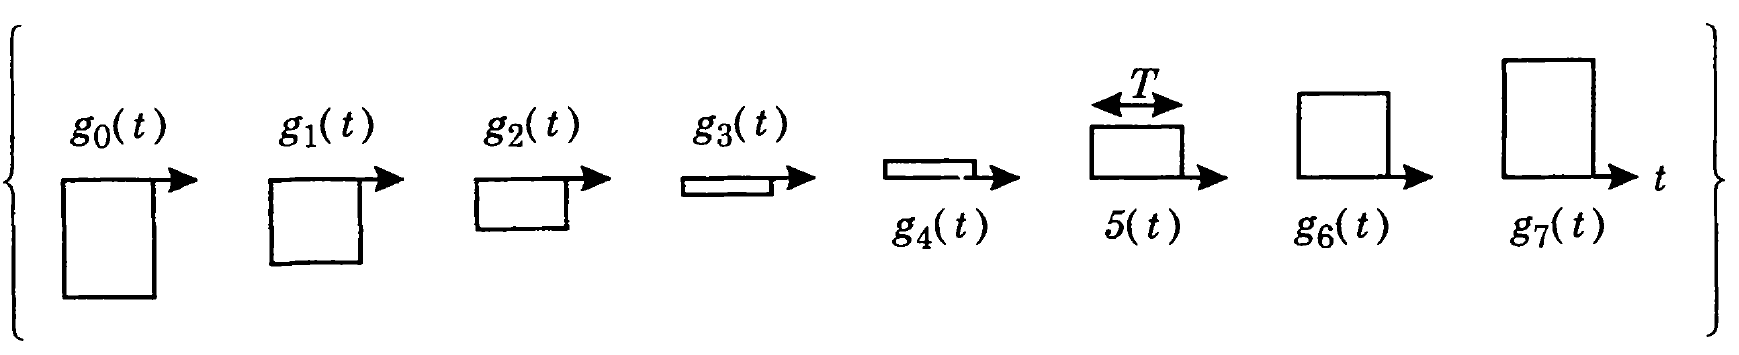
\includegraphics[width=0.75\columnwidth]{figs/adv_01}
	      \end{center}
	    \end{figure}
	\end{itemize}			
\end{frame}

\begin{frame}
	\frametitle{Modelo equivalente em banda base}

	\begin{itemize}
	    \item Relação entre sinal em banda passante $x(t)$ e sinal em banda base $s(t)$:
	    \begin{equation*}
		x(t) = \sqrt{2} \mathrm{Re}\{e^{j2\pi f_c t} s(t) \}
	    \end{equation*}
	    \item Similarmente para os pulsos em banda passante $\hat{g}(t)$ e banda base $g(t)$:
	    \begin{equation*}
		\hat{g}_i(t) = \sqrt{2} \mathrm{Re}\{e^{j2\pi f_c t} g_i(t) \}
	    \end{equation*}
	    \item Resultando no sinal em banda passante:
	     \begin{equation*}
		  x(t) = \sum_{k=-\infty}^{\infty} \hat{g}_{a_k}(t-kT)
	    \end{equation*}
	\end{itemize}			
\end{frame}

\begin{frame}
	\frametitle{Detecção de distância mínima}

	\begin{itemize}
	    \item Vamos considerar inicialmente a ausência de ISI, ou seja, assumindo que somente um pulso  é transmitido.
	    \item Um transmissor $M$-ário seleciona o sinal de $\{g_0(t), \ldots, g_{M-1}(t) \}$.
	    \item Supondo que $g_n(t)$ foi transmitido, o sinal recebido é dado por:
	    \begin{equation*}
		r(t) = h_n(t) + n(t)
	    \end{equation*}
	    \item Onde $h_n(t)$ é o $n$-ésimo pulso recebido e $n(t)$ é o ruído. Considerando que $b(t)$ é a resposta ao impulso do canal, temos:
	    \begin{equation*}
		H_n(f) = G_n(f)B(f+f_c)
	    \end{equation*}
	    \item Essa abordagem é válida para os casos em banda base e banda passante.
	\end{itemize}
\end{frame}

\begin{frame}
	\frametitle{Detecção de distância mínima}

	\begin{itemize}
	    \item Detector de distância mínima: escolhe o símbolo que melhor se aproxima ao sinal recebido.
	    \item Pode ser generalizado para o caso de modulação $M$-ária.
	    \item Função custo a ser \textcolor{blue}{minimizada}:
	    \begin{footnotesize}
	    \begin{equation*}
		J = \int_{-\infty}^{\infty} |r(t) - h_i(t)|^2 dt = \underbrace{\int_{-\infty}^{\infty} |r(t)|^2 dt}_{\mathcal{E}_r} - 2 \underbrace{\mathrm{Re}\left\{\int_{-\infty}^{\infty} r(t)h_i^*(t) dt \right\}}_{y_i} + \underbrace{\int_{-\infty}^{\infty} |h_i(t)|^2 dt}_{\mathcal{E}_i}
	    \end{equation*}
	    \end{footnotesize}
	    \item De forma análoga, o problema é equivalente a \textcolor{blue}{maximizar}:
	    \begin{equation*}
		 J_i = y_i - \frac{1}{2}\mathcal{E}_i
	    \end{equation*}
	    \item O que corresponde ao receptor de correlação.
	\end{itemize}
\end{frame}

\begin{frame}
	\frametitle{Detecção de distância mínima}

	\begin{itemize}
	    \item Ilustração do receptor de correlação:
	    \begin{figure}[t]	
	      \begin{center}
		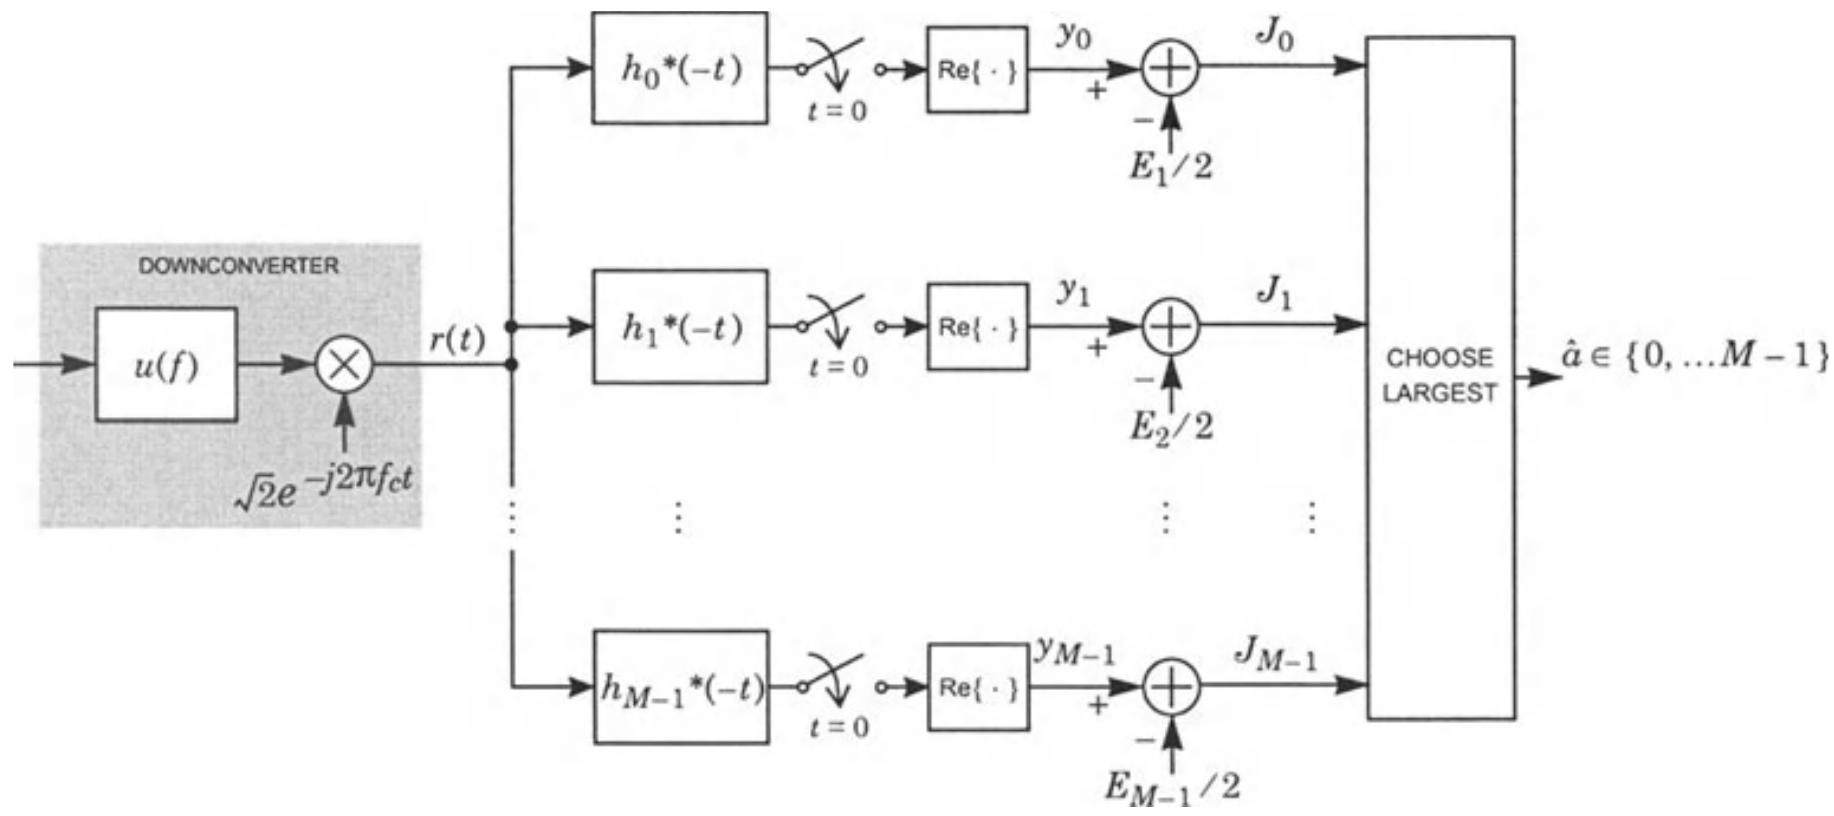
\includegraphics[width=0.85\columnwidth]{figs/adv_02}
	      \end{center}
	    \end{figure}
	    \item O sinal recebido é correlacionado com os $M$ possíveis pulsos utilizando um banco de filtros casados amostrados.
	\end{itemize}
\end{frame}

\begin{frame}
	\frametitle{Detecção de distância mínima}

	\begin{itemize}
	    \item Variação do receptor de correlação utilizando correlatores no lugar de filtros casados.
	    \begin{figure}[t]	
	      \begin{center}
		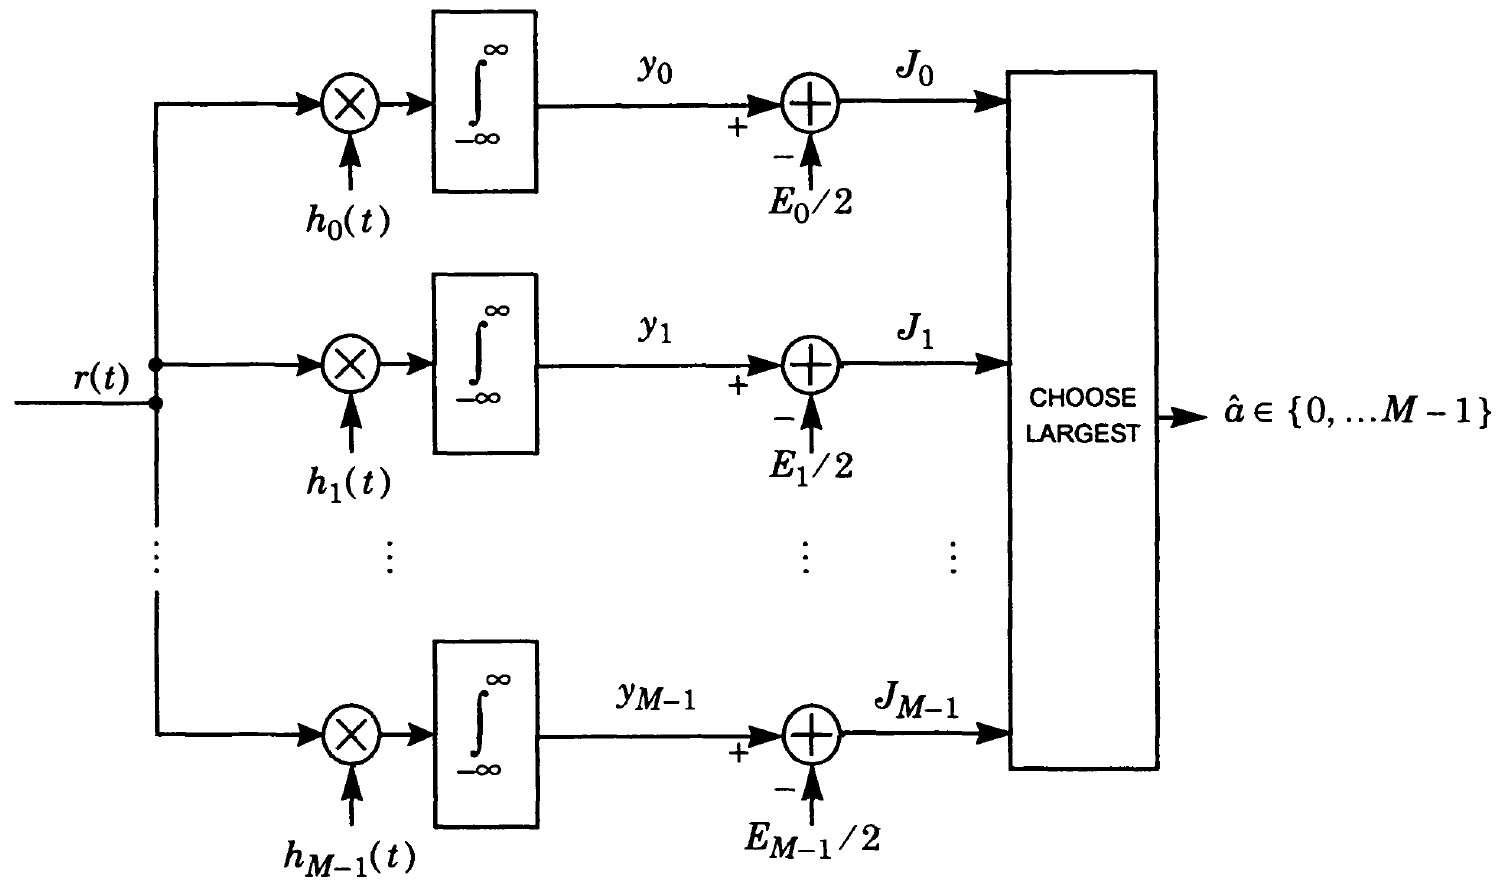
\includegraphics[width=0.7\columnwidth]{figs/adv_03}
	      \end{center}
	    \end{figure}
	    \item Adequado para cenário em banda base.
	\end{itemize}
\end{frame}

\begin{frame}
	\frametitle{Detecção de distância mínima}

	\begin{itemize}
	    \item Complexidade do receptor de correlação é dominada pelas $M$ correlações que devem ser computadas.
	    \item Motivação para se desenvolver um método de menor complexidade.
	    \item Seja $\mathcal{S} = \mathrm{span}\{h_0(t),\ldots,h_{M-1}(t) \}$ o \textcolor{blue}{espaço de sinal} e seja $\hat{r}(t)$ a projeção de $r(t)$ em $\mathcal{S}$.
	    \item Como o erro de projeção $r(t)-\hat{r}(t)$ é ortogonal a $\mathcal{S}$, temos:
	    \begin{align*}
		J &= \int_{-\infty}^{\infty}|r(t) - \hat{r}(t) + \hat{r}(t) - h_i(t)|^2 dt \\
		&= \int_{-\infty}^{\infty}|r(t) - \hat{r}(t)|^2 dt + \int_{-\infty}^{\infty}|\hat{r}(t) - h_i(t)|^2 dt
	    \end{align*}
	    \item O problema de otimização se reduz a minimizar:
	    \begin{equation*}
		J' = \int_{-\infty}^{\infty} |\hat{r}(t) - h_i(t)|^2 dt
	    \end{equation*}

	\end{itemize}
\end{frame}

\begin{frame}
	\frametitle{Detecção de distância mínima}

	\begin{itemize}
	    \item Seja $\{\phi_1(t),\ldots,\phi_N(t) \}$ uma base ortonormal para $\mathcal{S}$.
	    \item Pode-se utilizar o método de Gram-Schmidt sobre $\{h_0(t),\ldots,h_{M-1}(t) \}$.
	    \item Seja $\mathbf{h}_i = [h_{i,1}, h_{i,2},\ldots,h_{i,N}]^T$ o vetor de coeficientes da projeção de $h_i(t)$, onde:
	    \begin{equation*}
		h_{i,j} = \int_{-\infty}^{\infty} h_i(t)\phi_j^*(t) dt
	    \end{equation*}
	    \item O custo de distância mínima se reduz a:
	    \begin{equation*}
		J' = || \mathbf{r} - \mathbf{h}_i ||^2
	    \end{equation*}
	    \item Onde $\mathbf{r} = [r_1,\ldots,r_N]^T$ é o vetor projeção de $r(t)$, com:
	    \begin{equation*}
		r_j = \int_{-\infty}^{\infty} r(t)\phi_j^*(t) dt
	    \end{equation*}
	\end{itemize}
\end{frame}

\begin{frame}
	\frametitle{Detecção de distância mínima}

	\begin{itemize}
	    \item Forma alternativa de implementar o receptor de distância mínima: \textbf{Receptor de projeção}.    
	    \begin{figure}[t]	
	      \begin{center}
		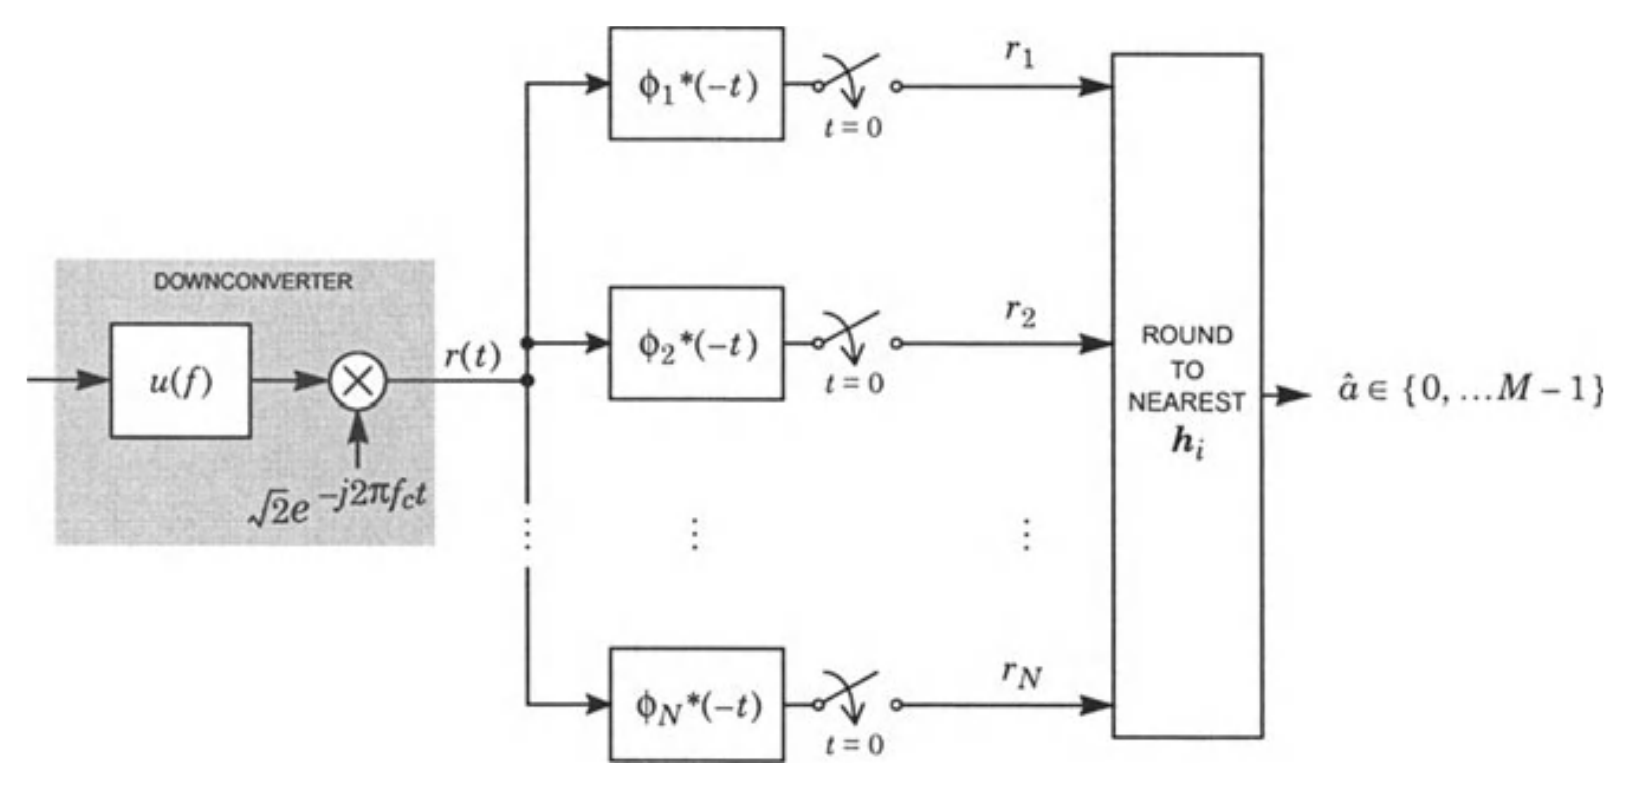
\includegraphics[width=0.75\columnwidth]{figs/adv_04}
	      \end{center}
	    \end{figure}
	    \item Complexidade reduzida de $M$ (tamanho da constelação) para $N$ (tamanho do espaço de sinal).
	\end{itemize}
\end{frame}

\section{Probabilidade de erro}

\begin{frame}
	\frametitle{Desempenho em cenário AWGN}

	\begin{itemize}
	    \item A $i$-ésima componente da projeção do sinal recebido é dada por:
	    \begin{equation*}
		    r_j = \underbrace{\int_{-\infty}^{\infty} h_i(t)\phi_j^*(t) dt}_{h_{i,j}} + \underbrace{\int_{-\infty}^{\infty} n(t)\phi_j^*(t) dt}_{n_j}
	    \end{equation*}
	    \item Considerando o vetor do ruído projetado $\mathbf{n}=[n_1,\ldots,n_N]^T$, temos:
	    \begin{equation*}
		    \mathbf{r} = \mathbf{h}_i + \mathbf{n}
	    \end{equation*}
	    \item $n(t)$ é a envoltória complexa do ruído Gaussiano branco em banda passante $\hat{n}(t)$. A DEP de $\hat{n}(t)$ é $N_0/2$ e a DEP de $n(t)$ é $N_0$.
	    \item Os $M$ vetores $\{\mathbf{h}_1,\ldots,\mathbf{h}_M \}$ são chamados de \textcolor{blue}{vetores de sinal}.
	\end{itemize}
\end{frame}

\begin{frame}
	\frametitle{Desempenho em cenário AWGN}

	\begin{itemize}
	    \item Podemos mostrar que as componentes do vetor $\mathbf{n}$ são i.i.d. com distribuição $\mathcal{CN}(0,N_0)$.
	    \item As componentes possuem média zero e a autocorrelação é dada por:
	    \begin{align*}
		\mathrm{E}[n_i n_j^*] = \mathrm{E}\left[\int_{-\infty}^{\infty} n(t)\phi_i^*(t) dt  \int_{-\infty}^{\infty} n^*(\tau)\phi_j(\tau) d\tau \right] = N_0 \delta_{i,j}
	    \end{align*}
	    \item Foram usadas as propriedades: linearidade da esperança, autocorrelação de $n(t)$ dada por $N_0\delta(t-\tau)$, e funções $\phi$ ortogonais entre si.
	    \item A matriz de autocorrelação de $\mathbf{n}$ é portanto diagonal.
	\end{itemize}
\end{frame}

\begin{frame}
	\frametitle{Desempenho em cenário AWGN}

	\begin{itemize}
	    \item Propriedades do vetor de ruído $\mathbf{n}$:
	    \begin{itemize}
		\item As $2N$ V.A.s reais $\{\mathrm{Re}\{n_1\},\ldots,\mathrm{Re}\{n_N\},\mathrm{Im}\{n_1\},\ldots,\mathrm{Im}\{n_N\} \}$ são mutuamente independentes, com média zero e variância $N_0/2$.
		\item O vetor $\mathbf{n}$ é circularmente simétrico e Gaussiano, com média zero e $\mathrm{E}[\mathbf{nn}^*] = N_0 \mathbf{I}$.
		\item Os componentes de $\mathbf{n}$ são descorrelacionados, $\mathrm{E}[n_in_j^*]=0$ para $i\neq j$.
		\item Os componentes de $\mathbf{n}$ são circularmente simétricos, $\mathrm{E}[n_in_j]=0$ para $1 \leq i, \; j\leq N$.
		\item Seja a variável aleatória $X = \langle \mathbf{n}, \mathbf{e} \rangle = \mathbf{e}^* \mathbf{n}$, ela será $\mathcal{CN}(0,N_0)$ para qualquer vetor $\mathbf{e}$ de norma unitária.
	    \end{itemize}
	\end{itemize}
\end{frame}

\begin{frame}
	\frametitle{Desempenho em cenário AWGN}

	\begin{itemize}
	    \item Normalmente não é possível encontrar o valor exato da probabilidade de erro do receptor de distância mínima.
	    \item Limitantes podem ser calculados para a probabilidade de erro.
	    \item \textcolor{blue}{Probabilidade de erro em pares} ($P_{i\rightarrow j}$):
	    \begin{itemize}
		\item Probabilidade de que o sinal recebido esteja mais próximo de $\mathbf{h}_j$ do que de $\mathbf{h}_i$, dado que $\mathbf{h}_i$ foi transmitido, para $j\neq i$.
	    \end{itemize}
	    \begin{align*}
		P_{i\rightarrow j} &= \mathrm{Pr}\left[ || \mathbf{r} - \mathbf{h}_j ||^2 < || \mathbf{r} - \mathbf{h}_i ||^2 \mid \mathbf{h}_i \text{ foi transmitido} \right] \\
		&= \mathrm{Pr}\left[ || \mathbf{n} - (\mathbf{h}_j - \mathbf{h}_i) ||^2 < || \mathbf{n} ||^2 \right] \\
		&= \mathrm{Pr}\Bigl[ || \mathbf{n} ||^2 + \underbrace{|| \mathbf{h}_j - \mathbf{h}_i ||^2}_{d_{i,j}^2} - 2\mathrm{Re}\{ \langle \mathbf{n}, \mathbf{h}_j - \mathbf{h}_i \rangle \} < || \mathbf{n} ||^2 \Bigr] \\
		&= \mathrm{Pr}\left[ \mathrm{Re}\{ \langle \mathbf{n}, (\mathbf{h}_j - \mathbf{h}_i)/d_{i,j} \rangle \} > d_{i,j}/2 \right] = Q\left(\frac{d_{i,j}}{2\sigma} \right)
	    \end{align*}
	\end{itemize}
\end{frame}

\begin{frame}
	\frametitle{Desempenho em cenário AWGN}

	\begin{itemize}
	    \item Comparação entre diferentes esquemas de modulação binária com mesma energia média $\mathcal{E}$.
	    \begin{figure}[t]	
	      \begin{center}
		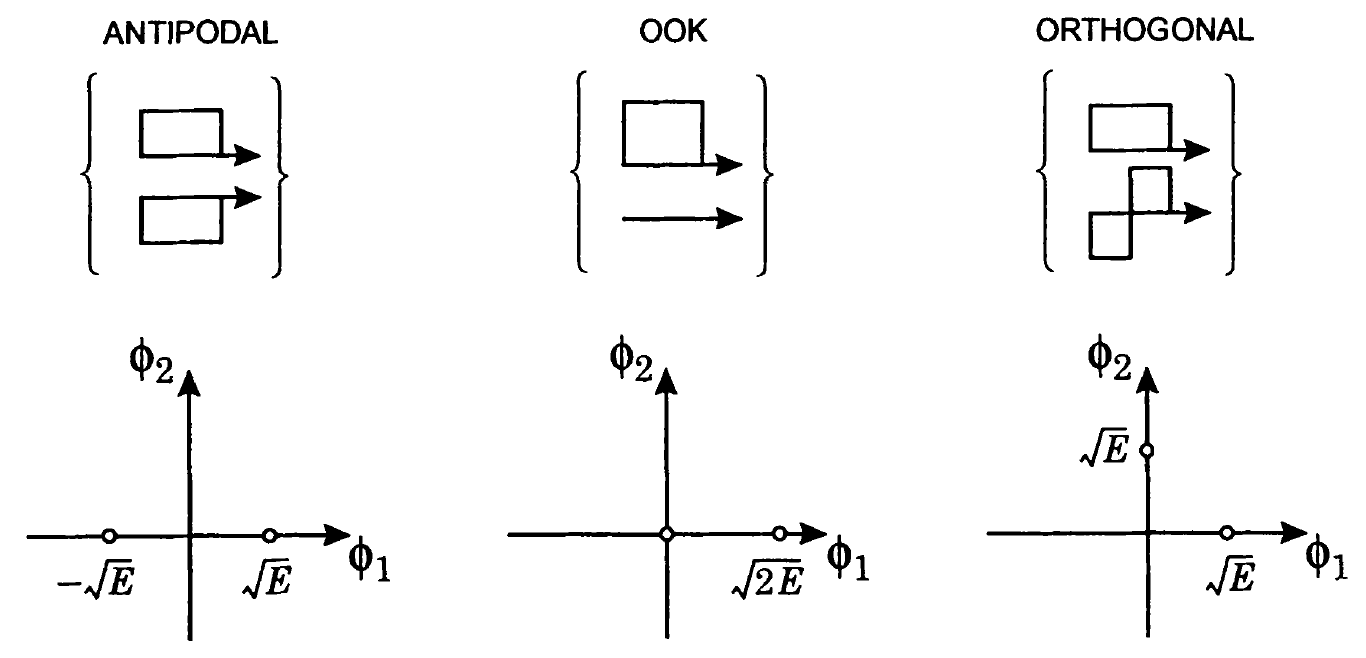
\includegraphics[width=0.65\columnwidth]{figs/adv_05}
	      \end{center}
	    \end{figure}
	    \item Sinalização antipodal: $d=2\sqrt{\mathcal{E}}$ e $P_e = Q(\sqrt{2\mathcal{E}/N_0})$
	    \item Sinalização OOK e ortogonal: $d=\sqrt{2\mathcal{E}}$ e $P_e = Q(\sqrt{\mathcal{E}/N_0})$
	    \item Vantagem de 3dB para a sinalização antipodal.
	\end{itemize}
\end{frame}

\begin{frame}
	\frametitle{Desempenho em cenário AWGN}

	\begin{itemize}
	    \item \textcolor{blue}{Limitante da união}: limitante superior para a probabilidade de erro.
	    \item De forma geral, para $N$ eventos de erro $\{ \mathpzc{E}_n, 1 \leq n \leq N \}$ temos
	    \begin{equation*}
		\mathrm{Pr}\left[ \bigcup_{n=1}^N \mathpzc{E}_n \right] \leq \sum_{n=1}^N \mathrm{Pr}[\mathpzc{E}_n] 
	    \end{equation*}
	    \item Considerando que $\mathbf{h}_0$ foi transmitido, podemos definir $\mathpzc{E}_j$ como o evento de erro no qual $\mathbf{h}_j$ é escolhido no lugar de $\mathbf{h}_0$, ou seja, $P_{0\rightarrow j} = \mathrm{Pr}[\mathpzc{E}_j]$.
	    \item Podemos então calcular o limitante superior:
	    \begin{align*}
		\mathrm{Pr}[\text{erro} \mid \mathbf{h}_0 \text{ foi transmitido}] &=  \mathrm{Pr}\left[ \bigcup_{j=1}^{M-1} \mathpzc{E}_j \right] \leq \sum_{j=1}^{M-1} \mathrm{Pr}[\mathpzc{E}_j] \\
		\mathrm{Pr}[\text{erro} \mid \mathbf{h}_0 \text{ foi transmitido}] &\leq \sum_{j=1}^{M-1} Q\left(\frac{d_{0,j}}{2\sigma} \right)
	    \end{align*}	    
	\end{itemize}
\end{frame}

\begin{frame}
	\frametitle{Desempenho em cenário AWGN}

	\begin{itemize}
	    \item O limitante inferior pode ser obtido considerando a probabilidade de um único evento $\mathpzc{E}_m$, para $1\leq m \leq M-1$.
	    \item Para que o limitante seja mais representativo, podemos considerar um evento de erro que tenha a mínima distância para o sinal transmitido.
	    \begin{equation*}
		 \mathrm{Pr}\left[ \bigcup_{j=1}^{M-1} \mathpzc{E}_j \right] \geq \mathrm{Pr}[\mathpzc{E}_{\min}] = Q\left(\frac{d_{0,\min}}{2\sigma} \right)
	    \end{equation*}
	    \item Chegamos portanto aos limitantes:
	    \begin{equation*}
		Q\left(\frac{d_{0,\min}}{2\sigma}\right) \leq \mathrm{Pr}[\text{erro} \mid \mathbf{h}_0 \text{ foi transmitido}] \leq  \sum_{j=1}^{M-1} Q\left(\frac{d_{0,j}}{2\sigma}\right)
	    \end{equation*}    
	\end{itemize}
\end{frame}

\begin{frame}
	\frametitle{Desempenho em cenário AWGN}

	\begin{itemize}
	    \item O limitante superior pode ser simplificado ao considerar somente os $K_0$ sinais que estão a uma distância $d_{0,\min}$ de $\mathbf{h}_0$.
	    \begin{equation*}
		\mathrm{Pr}[\text{erro} \mid \mathbf{h}_0 \text{ foi transmitido}] \approx K_0 Q\left(\frac{d_{0,\min}}{2\sigma}\right)
	    \end{equation*}
	    \item Neste caso deixa de ser um limitante superior, mas aproxima bem o valor da probabilidade para pequenos valores de $\sigma$.
	    \item Considerando $p_i$ como a probabilidade (\textit{a priori}) de um sinal ser transmitido, podemos calcular a probabilidade média de erro:
	    \begin{small}
	    \begin{equation*}
		P_e = \sum_{i=0}^{M-1} p_i \cdot \mathrm{Pr}[\mathbf{h}_i \text{ não escolhido} \mid \mathbf{h}_i \text{ transmitido}] \approx \sum_{i=0}^{M-1} p_i K_i Q\left(\frac{d_{i,\min}}{2\sigma}\right)
	    \end{equation*}
	    \end{small}
	\end{itemize}
\end{frame}

\begin{frame}
	\frametitle{Desempenho em cenário AWGN}

	\begin{itemize}
	    \item A expressão de $P_e$ pode ser simplificada considerando que o somatório será dominado pelos termos com menor argumento em $Q(\cdot)$.
	    \begin{equation*}
		P_e \approx K Q\left(\frac{d_{\min}}{2\sigma} \right)
	    \end{equation*}
	    \item Onde $d_{\min}$ é a distância mínima entre qualquer par de sinais.
	    \item $K$ é chamado de \textcolor{blue}{coeficiente de erro} e representa o número médio de sinais a uma distância mínima.
	\end{itemize}
\end{frame}

\section{Modulação ortogonal}

\begin{frame}
	\frametitle{Modulação ortogonal}

	\begin{itemize}
	    \item A \textcolor{blue}{modulação ortogonal} é um caso especial da modulação $M$-ária, na qual os sinais são ortogonais e possuem mesma energia.
	    \begin{equation*}
		\int_{-\infty}^{\infty} g_i(t)g_j^*(t) dt = \mathcal{E}_g \delta_{i-j}
	    \end{equation*}
	    \item Vamos assumir o caso sem ISI (e.g., pulsos satisfazendo o critério de Nyquist) e com canal benigno (e.g., resposta em frequência plana), desta forma a ortogonalidade dos pulsos recebidos se mantém.
	    \begin{equation*}
		\int_{-\infty}^{\infty} h_i(t)h_j^*(t) dt = \mathcal{E} \delta_{i-j}
	    \end{equation*}
	    \item Os sinais ortogonais possuem \textcolor{red}{baixa eficiência espectral}, pois o aumento da ordem da modulação requer recursos adicionais para garantir a ortogonalidade.
	\end{itemize}
\end{frame}

\begin{frame}
	\frametitle{Receptor de distância mínima para modulação ortogonal}

	\begin{itemize}
	    \item Os receptores mencionados anteriormente podem ser adaptados para a modulação ortogonal.
	    \item Como os pulsos são ortogonais, o processo de Gram-Schmidt resulta em um espaço de sinal com $N=M$.    
	    \item O receptor de projeção possui, portanto, a mesma complexidade que o receptor de correlação.
	\end{itemize}
	\begin{figure}[t]	
	    \begin{center}
	    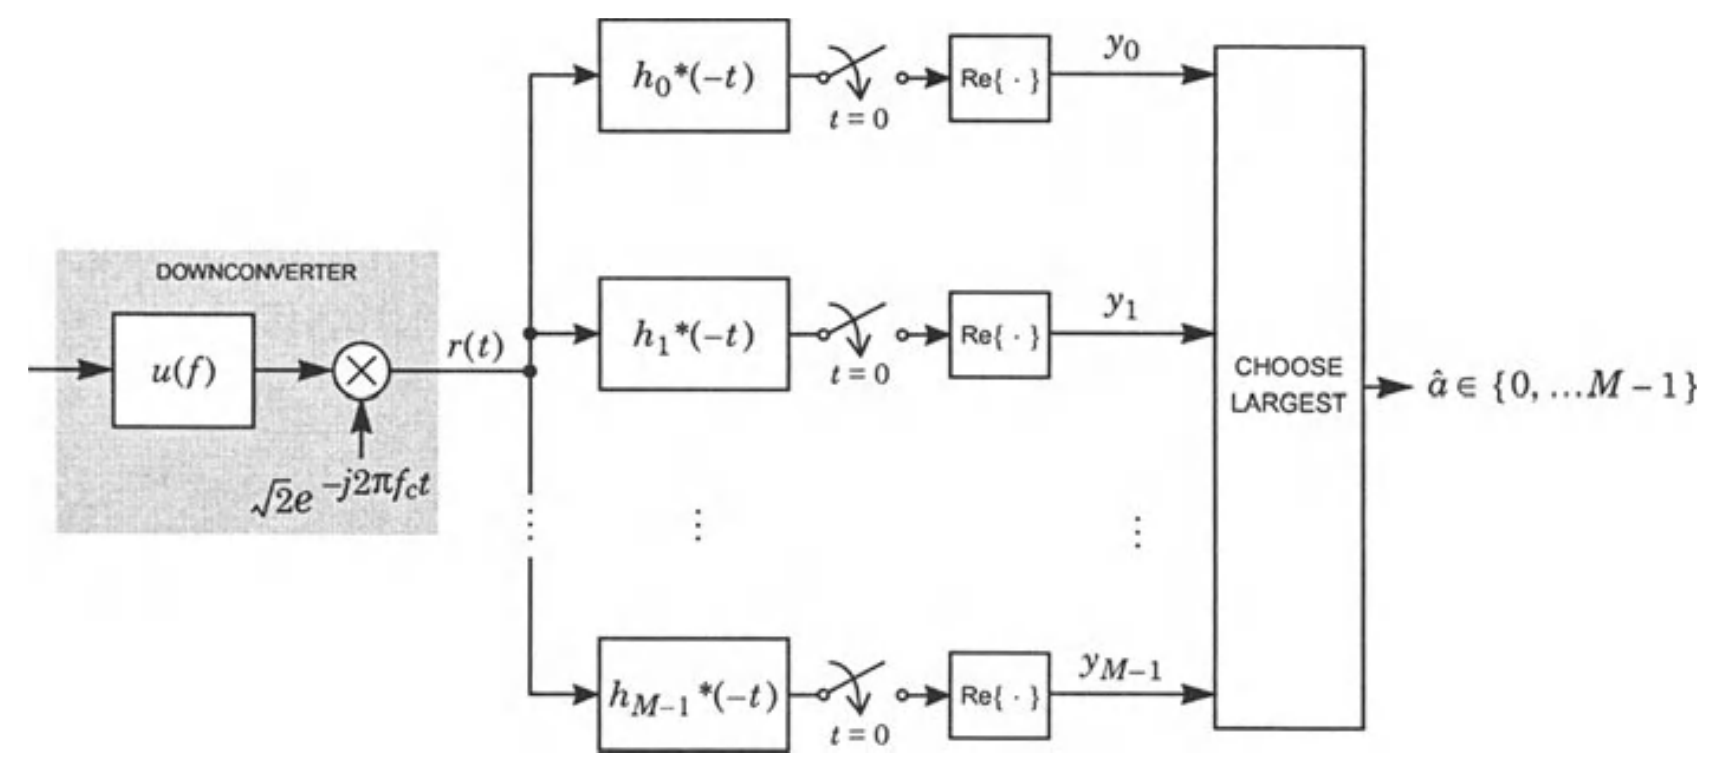
\includegraphics[width=0.7\columnwidth]{figs/adv_07}
	    \end{center}
	\end{figure}
\end{frame}

\begin{frame}
	\frametitle{Probabilidade de erro para modulação ortogonal}

	\begin{itemize}
	    \item Vetor projeção do sinal recebido na modulação ortogonal:
	    \begin{equation*}
		\mathbf{h}_i = [0, 0, \ldots, 0, \sqrt{\mathcal{E}}, 0, \ldots, 0]^T
	    \end{equation*}
	    \item Termo não-nulo está na $i$-ésima posição e $d=d_{\min}= \sqrt{2E}$.
	\end{itemize}
	\begin{columns}
	    \begin{column}{0.5\textwidth}
		\begin{itemize}
		    \item Probabilidade de erro aproximada:
		    \begin{align*}
			P_e &\approx (M-1) Q\left(\frac{d_{\min}}{2\sigma} \right) \\
			&\approx (M-1)Q\left(\sqrt{\frac{\mathcal{E}}{N_0}} \right)
		    \end{align*}
		    \item Aumento de $M$ impacta a banda, mas não o argumento de $Q(\cdot)$
		\end{itemize}		
	    \end{column}
	    \begin{column}{0.5\textwidth}
% 		\begin{itemize}
% 		    \item 
% 		\end{itemize}
		\begin{figure}[t]	
		    \begin{center}
		    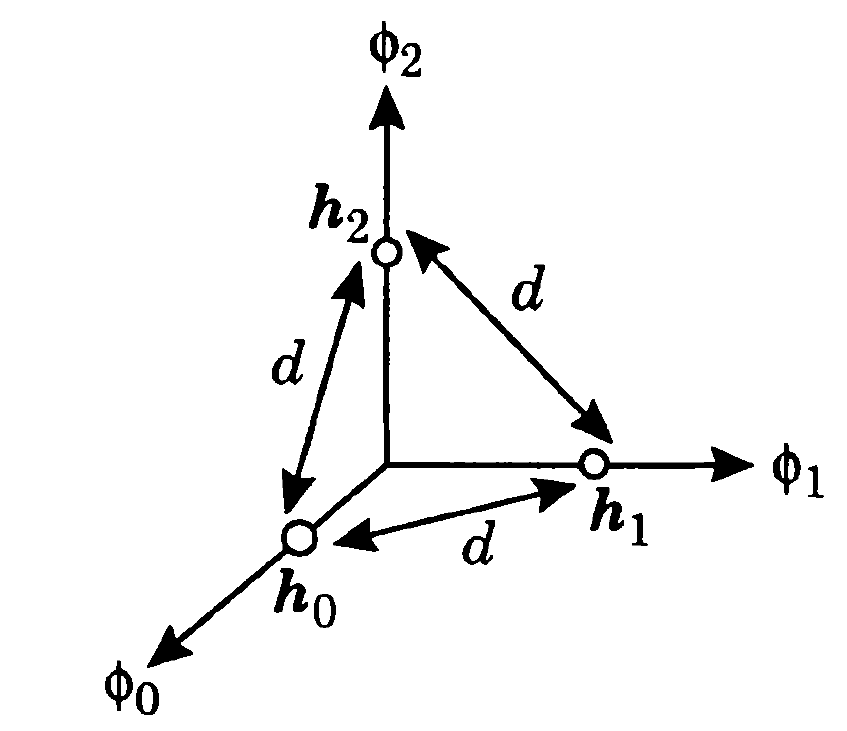
\includegraphics[width=0.6\columnwidth]{figs/adv_06}
		    \end{center}
		\end{figure}\vspace{-0.3cm}
		\centering \begin{small}Exemplo para $M$=3:\end{small}
	    \end{column}	    
	\end{columns}	
\end{frame}

\begin{frame}
	\frametitle{Probabilidade de erro para modulação ortogonal}

	\begin{itemize}
	    \item Probabilidade de erro não depende do sinal transmitido.
	    \item Cálculo da probabilidade exata de erro da modulação ortogonal:
	    \begin{alignat*}{2}
		&\mathrm{Pr}[\text{acerto}&& \mid \mathbf{h}_0 \text{ transmitido},y_0=y] = \left(1 - Q\left( \frac{y}{\sigma} \right) \right)^{M-1} \\
		&\mathrm{Pr}[\text{erro}] &&= \mathrm{Pr}[\text{erro} \mid \mathbf{h}_0 \text{ transmitido}] = 1 - \mathrm{Pr}[\text{acerto} \mid \mathbf{h}_0 \text{ transmitido}] \\
		& &&= 1 - \int_{-\infty}^{\infty} f_{y_0}(y) \left( 1 - Q\left(\frac{y}{\sigma} \right) \right)^{M-1} dy
	    \end{alignat*}
	    \item Onde $f_{y_0}(y)$ é a PDF Gaussiana, com média $\sqrt{\mathcal{E}}$ e variância $\sigma^2$
	\end{itemize}	
\end{frame}

\begin{frame}
	\frametitle{Probabilidade de erro para modulação ortogonal}

	\begin{itemize}
	    \item Curvas de probabilidade de erro:
	\end{itemize}	
	\begin{figure}[t]	
	    \begin{center}
	    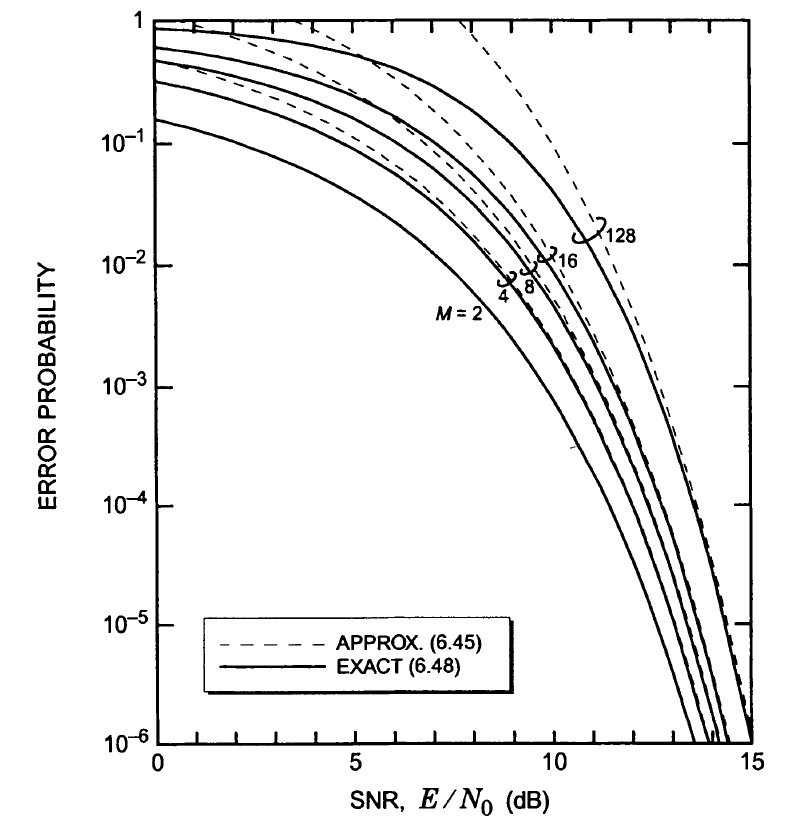
\includegraphics[width=0.5\columnwidth]{figs/adv_08}
	    \end{center}
	\end{figure}
\end{frame}

\begin{frame}
	\frametitle{Exemplos de modulação ortogonal}

	\begin{itemize}
	    \item Formas canônicas:
	    \begin{itemize}
	     \item Chaveamento de frequência: Frequency Shift Keying (FSK)
	     \item Modulação por posição de pulso: Pulse Position Modulation (PPM)
	    \end{itemize}
	    \item Exemplo de um sinal FSK binário e esquema de detecção:
	    \begin{figure}[t]	
		\begin{center}
		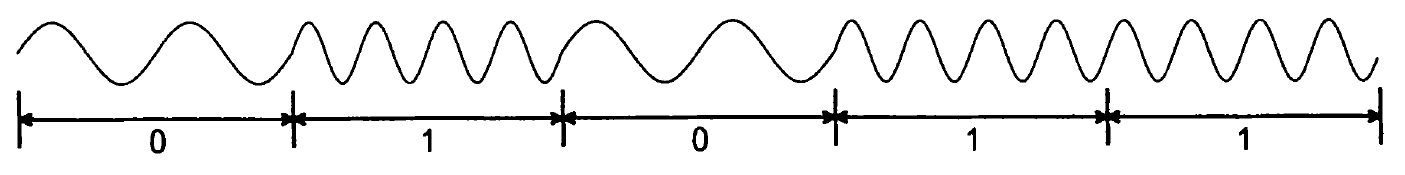
\includegraphics[width=0.75\columnwidth]{figs/adv_09}
		\end{center}
	    \end{figure}
	    \begin{figure}[t]	
		\begin{center}
		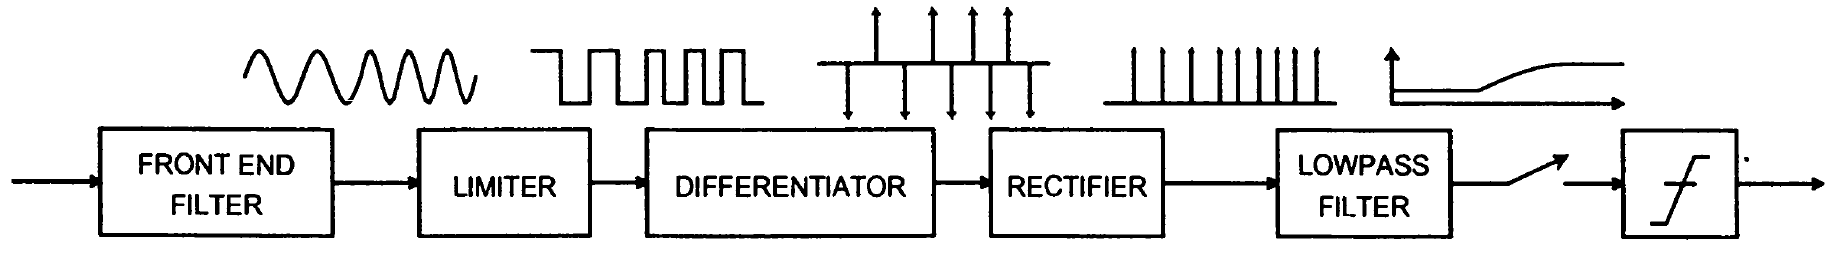
\includegraphics[width=0.75\columnwidth]{figs/adv_10}
		\end{center}
	    \end{figure}	    
	    \item Vantagens do FSK: incoerência (não é necessária detecção de fase), facilidade de implementação, imunidade a certas não-linearidades.
	    \item Desvantagens do FSK: baixa eficiência espectral, penalidade de 3 dB em relação ao PAM antipodal, dificuldade em compensar distorções.
	\end{itemize}	
\end{frame}

\begin{frame}
	\frametitle{Exemplos de modulação ortogonal}

	\begin{itemize}
	    \item Exemplo de modulação FSK usando pulso em formato sinc:
	    \begin{equation*}
		h_n(t) = \sqrt{\frac{\mathcal{E}}{T}}\left( \frac{\sin(\pi t / (2T))}{\pi t/(2T)} \right) \cos \left( (n+ 1/2) \frac{\pi t}{T} \right)
	    \end{equation*}
	    \item Pulsos no tempo e frequência, para $n=1,\ldots,4$
	    \begin{figure}[t]	
		\begin{center}
		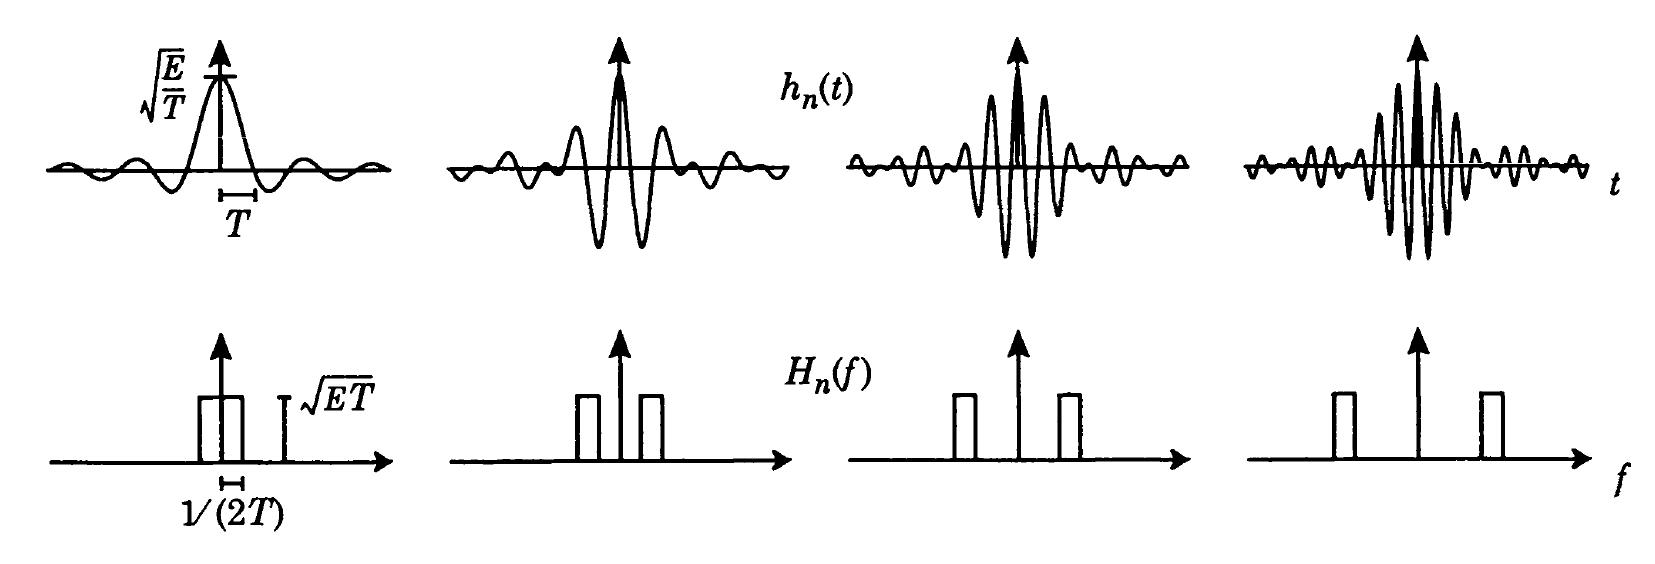
\includegraphics[width=0.85\columnwidth]{figs/adv_11}
		\end{center}
	    \end{figure}
	    \item Pulso ortogonal com energia $\mathcal{E}$ e banda $1/(2T)$.
	\end{itemize}	
\end{frame}

\begin{frame}
	\frametitle{Exemplos de modulação ortogonal}

	\begin{itemize}
	    \item Modulação por posição de pulso (PPM) divide o intervalo de sinalização em $M$ \textit{slots} de largura $T/M$.
	    \item Envia o pulso em um dos \textit{slots}, carregando $\log_2 M$ bits de informação.
	    \item Conjunto PPM $M$-ário: $\{g(t), g(t-T/M), \ldots, g(t-(M-1)T/M) \}$.
	    \item Exemplos do 4-PPM com pulso: (a) retangular e (b) de banda mínima.
	    \begin{figure}[t]	
		\begin{center}
		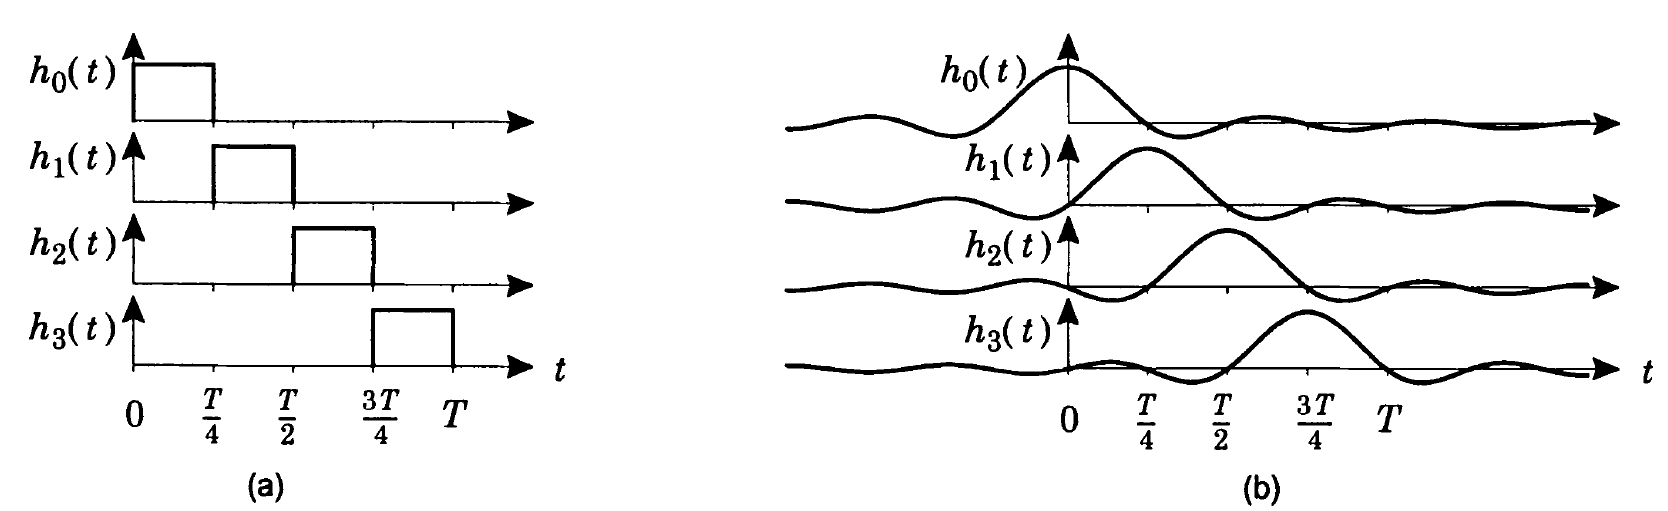
\includegraphics[width=0.8\columnwidth]{figs/adv_12}
		\end{center}
	    \end{figure}
	    \item Pulso de banda mínima: $g(t) = \sqrt{\mathcal{E}M/T}\sin(M\pi t)/(M\pi t/T)$
	    \item Pulso ortogonal com energia $\mathcal{E}$ e banda $1/(2T)$.
	\end{itemize}	
\end{frame}

\begin{frame}
	\frametitle{Critério de Nyquist generalizado}

	\begin{itemize}
	    \item Para o PAM com tempo de símbolo $T$, a banda mínima é $1/(2T)$.
	    \item O critério de Nyquist pode ser generalizado para modulações ortogonais.
	    \item Dado um conjunto de $M$ sinais ortogonais, o critério de banda mínima é dado por $M/(2T)$ Hz para o conjunto de sinais.
	    \item O requisito de banda aumenta com o tamanho da constelação.
	    \item Considerando um receptor com filtro casado amostrado, dado um sinal de entrada $h_i(t)$, as amostras na saída do filtro devem satisfazer o critério de Nyquist para evitar ISI:	    
	    \begin{equation*}
		h_i(t) * h_i^*(-t) \mid_{t=kT} = \delta_k \, , \qquad 0 \leq i \leq M-1
	    \end{equation*}
	    \item Critério adicional para evitar interferência entre os diferentes pulsos:
	    \begin{equation*}
		h_i(t) * h_j^*(-t) \mid_{t=kT} = 0 \, , \quad j\neq i \qquad -\infty \leq k \leq \infty
	    \end{equation*}
	\end{itemize}	
\end{frame}

\begin{frame}
	\frametitle{Critério de Nyquist generalizado}

	\begin{itemize}
	    \item Combinação das duas condições:
	    \begin{equation*}
		h_i(t) * h_j^*(-t) \mid_{t=kT} = \delta_k\delta_{j-i}
	    \end{equation*}
	    \item Seja $H_i(f)$ a transformada de Fourier de $h_i(t)$, podemos expressar o \textcolor{blue}{critério generalizado de Nyquist}:
	    \begin{equation*}
		\frac{1}{T}\sum_{m=-\infty}^{\infty} H_i\left(f-\frac{m}{T} \right) H_j^*\left(f-\frac{m}{T} \right) = \delta_{j-i}
	    \end{equation*}
	    \item Uma banda de $M/(2T)$ é condição necessária e suficiente para satisfazer o critério, como ilustrado nos casos do FSK e PPM.
	\end{itemize}	
\end{frame}

\begin{frame}
	\frametitle{Critério de Nyquist generalizado}

	\begin{itemize}
	    \item O pulso ideal possui problemas de realizabilidade: necessário projeto de pulsos práticos que possuam banda próxima da mínima.
	    \item Seja $w(t)$ um pulso tal que $w(t)*w(-t)$ (saída do filtro casado) satisfaz o critério de Nyquist para uma taxa $1/(2T)$.
	    \begin{equation*}
		\int_{-\infty}^{\infty} w(t) w(t-2kT)dt = \delta_k \qquad \text{(\textcolor{blue}{C1})}
	    \end{equation*}
	    \item A banda mínima de $w(t)$ é $1/(4T)$, mas para permitir um decaimento suave vamos assumir o dobro da banda mínima, $1/(2T)$.
	    \item Obtenção de um conjunto de $M$ pulsos ortogonais a partir de $w(t)$, para $n\in \{0,\ldots, M-1 \}$:
	    \begin{equation*}
		h_n(t) = w(t) \cos \left( (n+3/2) \frac{\pi t}{T} \right) 
	    \end{equation*}
	\end{itemize}	
\end{frame}

\begin{frame}
	\frametitle{Critério de Nyquist generalizado}

	\begin{itemize}
	    \item Exemplo de pulso cuja magnitude $|W(f)|^2$ satisfaz o critério de Nyquist:
	    \begin{figure}[t]	
		\begin{center}
		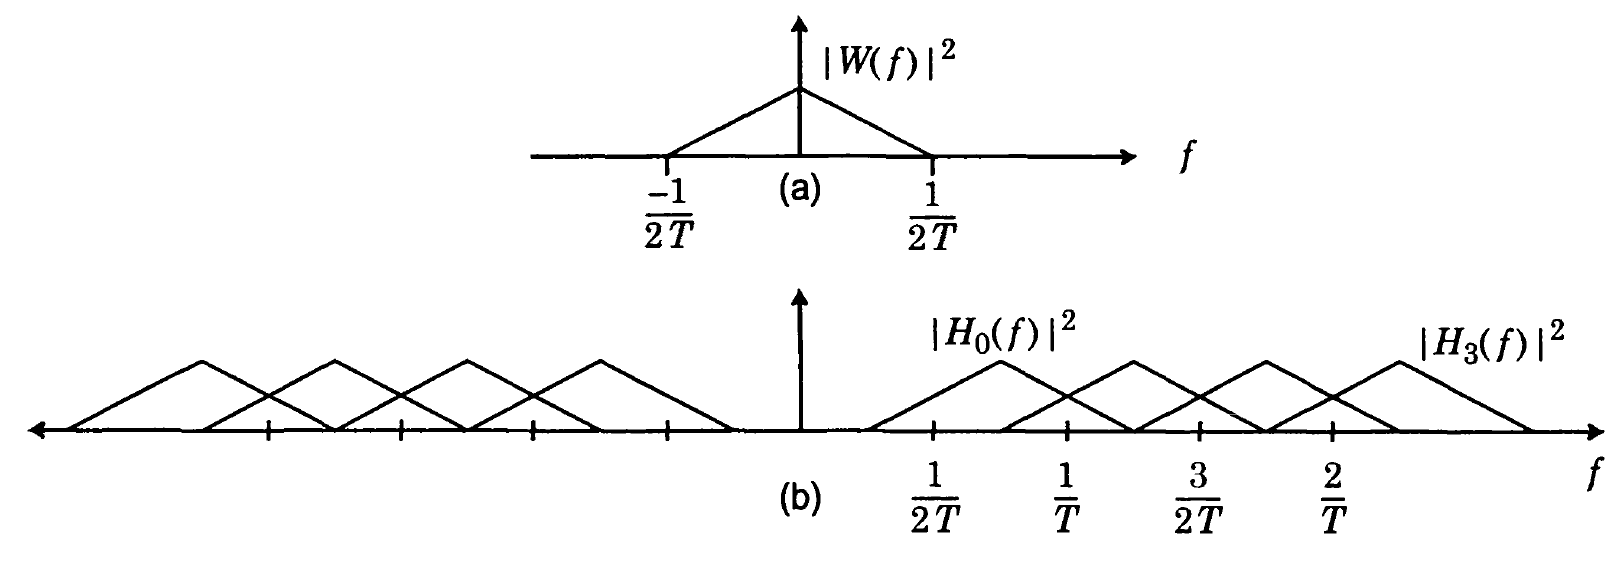
\includegraphics[width=0.8\columnwidth]{figs/adv_13}
		\end{center}
	    \end{figure}
	    \item O conjunto $h_n(t)$ satisfaz o critério de Nyquist generalizado se:
	    \begin{equation*}
		\mathrm{Re}\{W(f) W(1/(2T)-f) \} = 0 \, , \qquad 0 \leq f \leq 1/(4T) \qquad \text{(\textcolor{blue}{C2})}
	    \end{equation*}
	    \item Essa condição pode ser satisfeita se a fase de $W(f)$ apresentar uma simetria específica em torno de $1/(4T)$.
	\end{itemize}	
\end{frame}

\begin{frame}
	\frametitle{Critério de Nyquist generalizado}

	\begin{itemize}
	    \item O projeto de $W(f)$ pode ser feito satisfazendo as condições (\textcolor{blue}{C1}) para a magnitude e (\textcolor{blue}{C2}) para a fase.
	    \item Considerando $W(f) = A(f) e^{j\theta(f)}$, temos que:
	    \begin{small}
	    \begin{equation*}
		  \mathrm{Re}\{W(f) W(1/(2T)-f) \} = A(f)A(1/(2T)-f)\cos\left(\theta(f)+\theta(1/(2T)-f) \right)
	    \end{equation*}
	    \end{small}
	    \item Essa função se anula para todo $0\leq f \leq 1/(4T)$ se
	    \begin{equation*}
		  \theta(f) + \theta(1/(2T)-f) = \pm \pi/2
	    \end{equation*}
	    \item Exemplo de função que satisfaz essa restrição:
	    \begin{equation*}
		  \theta(f) = -\pi fT + \gamma(f)
	    \end{equation*}
	    \item Onde $\gamma(f)$ possui simetria ímpar em torno de $1/(4T)$.
	\end{itemize}	
\end{frame}

\begin{frame}
	\frametitle{Critério de Nyquist generalizado}

	\begin{itemize}
	    \item Foi definido um conjunto de pulsos que satisfaz o critério generalizado de Nyquist.
	    \item Magnitude de $W(f)$: escolhida de forma que $w(t)*w(-t)$ satisfaça o critério convencional de Nyquist a uma taxa $1/(2T)$.
	    \item Fase de $W(f)$: escolhida de forma a forçar a ortogonalidade dos pulsos.
	    \item Os pulsos $\{h_0(t),\ldots,h_{M-1}(t) \}$ cobrem o intervalo de frequências $[1/(4T), (2M+3)/(4T)]$
	    \item Banda total de $(M+1)/(2T)$, ligeiramente superior ao mínimo $M/(2T)$.
	\end{itemize}	
\end{frame}

\begin{frame}
	\frametitle{Imunidade ao ruído e eficiência espectral}

	\begin{itemize}
	    \item O mapeamento Gray não se aplica à modulação ortogonal, pois todos os símbolos estão à mesma distância uns dos outros.
	    \item Qualquer mapeamento resultará na mesma probabilidade de erro de bit.
	    \item Suponha que um dado sinal é transmitido e considere os $M-1$ vizinhos, cada um com uma combinação de bits de tamanho $b=\log_2 M$ bits.
	    \item Os símbolos adjacentes não diferem somente em um bit.
	    \item Diferenças de $k$ bits: $\binom{b}{k}$	    
	    \item Assumindo sinais equiprováveis, a probabilidade de um erro específico de símbolo é $P_e/(M-1)$.
	    \item Calculando a média em $k\in \{1,\ldots,b \}$ obtemos a probabilidade média de erro de bit:
	    \begin{equation*}
		P_b = \frac{\sum\limits_{k=1}^b \binom{b}{k}\frac{P_e}{M-1}}{b} = \frac{M/2}{M-1}P_e
	    \end{equation*}	
	\end{itemize}	
\end{frame}

\begin{frame}
	\frametitle{Imunidade ao ruído e eficiência espectral}

	\begin{itemize}
	    \item Energia por bit: $\mathcal{E}_b = \mathcal{E} / (\log_2 M)$.
	    \item Aproximação da probabilidade de erro de bit:
	    \begin{equation*}
		  P_b \approx \frac{M}{2}Q\left(\sqrt{\log_2 M \frac{\mathcal{E}_b}{N_0} } \right)
	    \end{equation*}
	    \item Requisito de SNR por bit:
	    \begin{equation*}
		  \mathcal{E}_b/N_0 = \frac{\left( Q^{-1}\left( \frac{P_b}{M/2} \right) \right)^2}{\log_2 M}
	    \end{equation*}
	    \item Como a banda mínima é dada por $M/(2T)$, a melhor eficiência espectral é dada por:
	    \begin{equation*}
		    \nu = \frac{\log_2 M}{T(M/2T)} = \frac{2\log_2 M}{M}
	    \end{equation*}
	\end{itemize}
\end{frame}

\begin{frame}
	\frametitle{Imunidade ao ruído e eficiência espectral}

	\begin{itemize}
	    \item Diferenciando $\nu$ com relação a $M$, encontramos que o máximo é alcançado para $M=e$.
	    \item Desempenho da modulação ortogonal.
	\end{itemize}
	\begin{figure}[t]	
	    \begin{center}
	    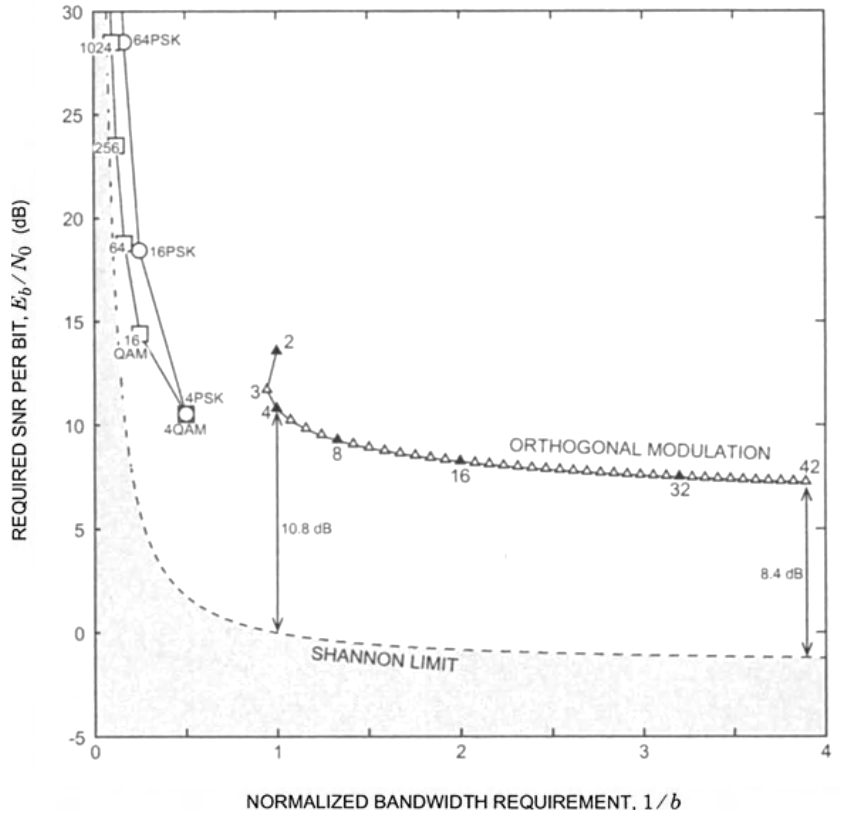
\includegraphics[width=0.51\columnwidth]{figs/adv_14}
	    \end{center}
	\end{figure}
\end{frame}

\begin{frame}
	\frametitle{Questões práticas do FSK}

	\begin{itemize}
	    \item O FSK pode ter fase contínua ou descontínua:
	    \begin{figure}[t]	
		\begin{center}
		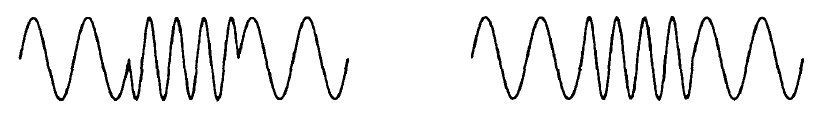
\includegraphics[width=0.65\columnwidth]{figs/adv_15}
		\end{center}
	    \end{figure}
	    \item Fase contínua é desejável, pois reduz os componentes de alta frequência.
	    \item Condição de fase contínua: cada pulso deve percorrer um número inteiro $M_i$ de ciclos.
	    \begin{equation*}
		f_iT = M_i
	    \end{equation*}
	    \item Separação mínima entre as frequências também é desejável.
	    \item Para que seja mantida a continuidade de fase e a ortogonalidade, a separação mínima é dada por:
	    \begin{equation*}
		f_i - f_{i-1} = 1/T \, , \qquad 1 \leq i \leq M-1
	    \end{equation*}
	\end{itemize}	
\end{frame}

\begin{frame}
	\frametitle{Questões práticas do FSK}

	\begin{itemize}
	    \item O filtro casado e receptor de correlação exigem conhecimento exato da frequência e fase (receptores coerentes).
	    \item FSK permite usar de forma prática um receptor não-coerente.
	\end{itemize}	
	\begin{figure}[t]	
	    \begin{center}
	    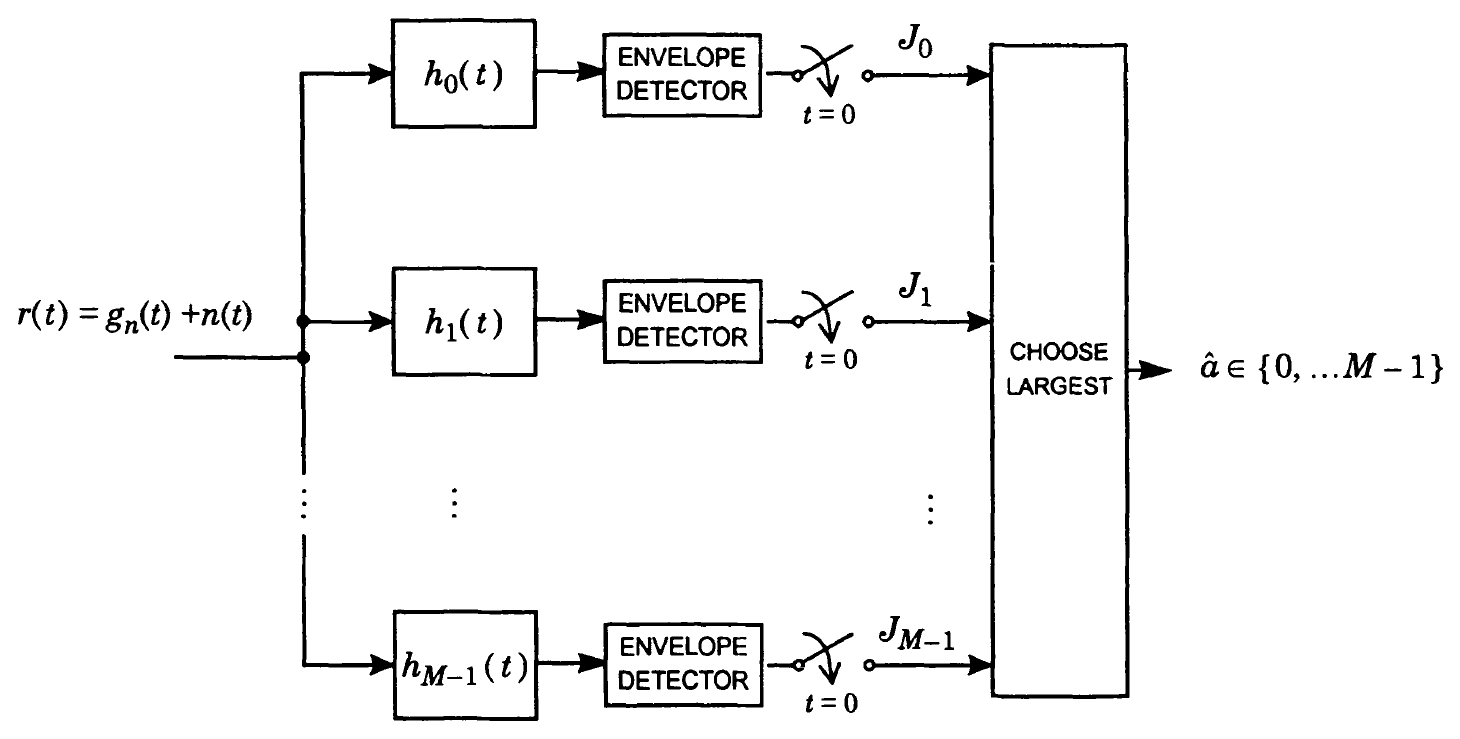
\includegraphics[width=0.8\columnwidth]{figs/adv_18}
	    \end{center}
	\end{figure}
\end{frame}

% \section{PAM ortogonal (OPAM)}
% 
% \begin{frame}
% 	\frametitle{PAM ortogonal (OPAM)}
% 
% 	\begin{itemize}
% 	    \item 
% 	\end{itemize}	

% \end{frame}

\section{Modulação com memória}

\begin{frame}
	\frametitle{Modulação com memória}

	\begin{itemize}
	    \item Até agora consideramos esquemas sem memória, ou seja, o sinal transmitido durante o $k$-ésimo intervalo de sinalização não depende de símbolos anteriores.
	    \item Vamos generalizar o modulador para também levar em conta símbolos anteriores na determinação do sinal transmitido.
	    \item Tipos comuns de modulação com memória:
	    \begin{itemize}
		\item Modulação de fase contínua (CPM)
		\item Chaveamento de mínimo deslocamento (MSK)
		\item Modulação diferencial
	    \end{itemize}
	\end{itemize}	
\end{frame}

\begin{frame}
	\frametitle{Modulação de fase contínua}

	\begin{itemize}
	    \item Um modulador FSK de fase contínua pode ser implementado utilizando um oscilador de fase controlado por tensão (VCO):
	    \begin{figure}[t]	
		\begin{center}
		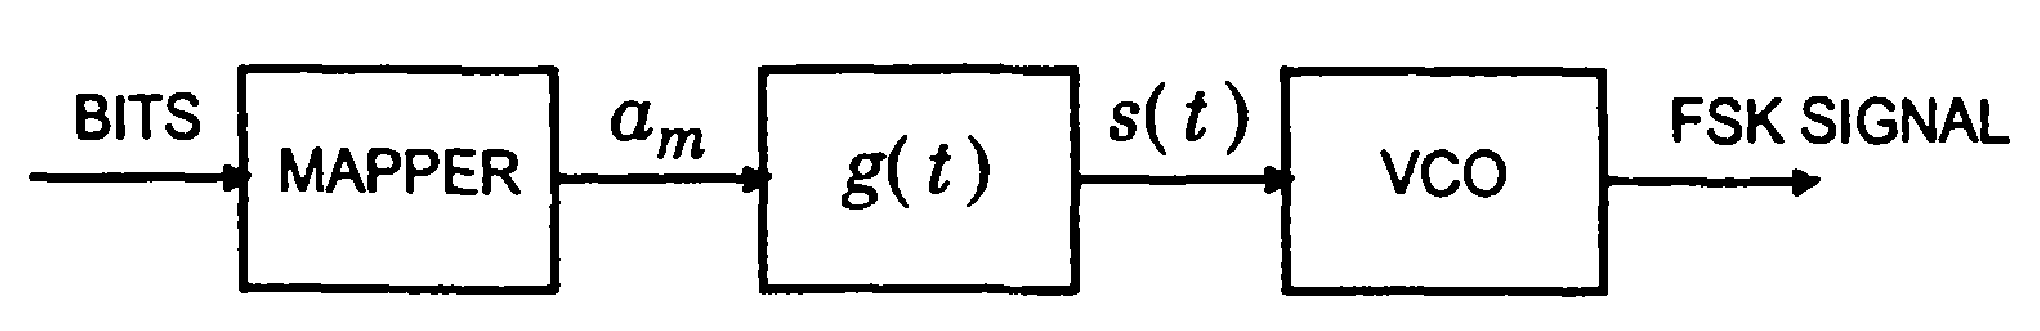
\includegraphics[width=0.7\columnwidth]{figs/adv_23}
		\end{center}
	    \end{figure}
	    \item A frequência do VCO varia em torno de $f_c$, mantendo automaticamente a continuidade da fase.
	    \item Sinal modulado de fase contínua (CPM), antes e após o VCO:
	    \begin{align*}
		 s(t) &= \sum_{k=-\infty}^{\infty} a_k g(t-kT) \\
		 x(t) &= K \cos\left[2\pi \left( f_c t + f_d \int_{-\infty}^t s(\tau) d\tau \right) \right]
	    \end{align*}
	\end{itemize}	
\end{frame}

\begin{frame}
	\frametitle{Modulação de fase contínua}

	\begin{itemize}
	    \item Quando o sinal $s(t)$ é normalizado para $|s(t)|\leq 1$, o fator $f_d$ corresponde ao valor de pico do desvio de frequência.
	    \item Para $g(t)$ retangular, o CPM se torna: FSK de fase contínua (CPFSK).
	    \item A largura de banda do FSK normalmente é maior que a do PAM para uma mesma taxa de símbolo.
	    \item O chaveamento de mínimo deslocamento (MSK) permite reduzir o requisito de banda.
	    \item O MSK obtém um desvio de frequência $f_d$ de metade do valor do FSK convencional.
	\end{itemize}	
\end{frame}

\begin{frame}
	\frametitle{Chaveamento de mínimo deslocamento (MSK)}

	\begin{itemize}
	    \item Para o FSK a separação em frequência deve ser igual à taxa de símbolo $1/T$, para o MSK a separação cai para a metade:
	    \begin{equation*}
		f_i - f_{i-1} = 1/(2T) \, , \qquad 1 \leq i \leq M-1
	    \end{equation*}
	    \item Exemplo de modulação MSK binária com $f_d = 1/(4T)$:
	    \begin{figure}[t]	
		\begin{center}
		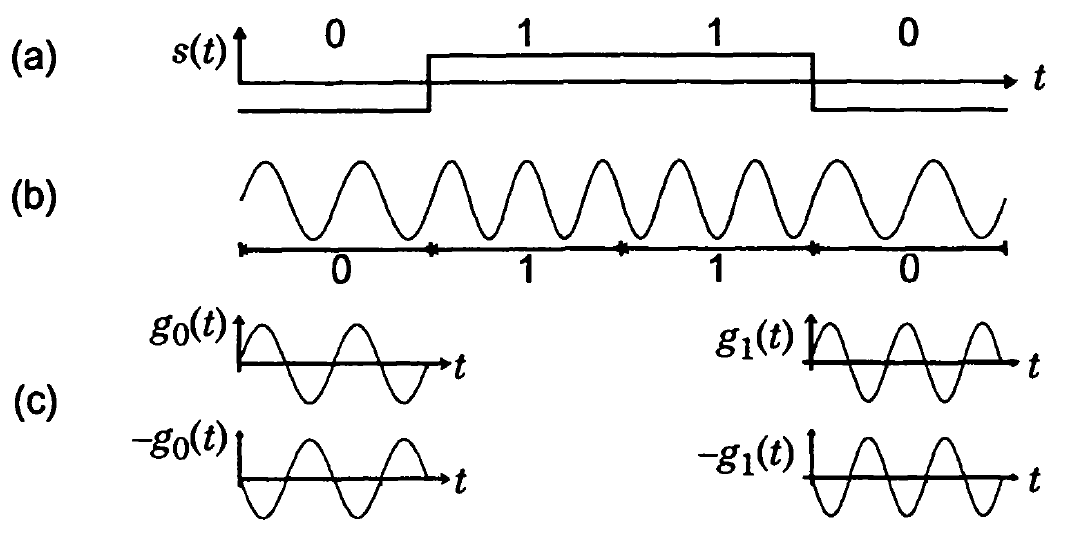
\includegraphics[width=0.6\columnwidth]{figs/adv_25}
		\end{center}
	    \end{figure}
	\end{itemize}	
\end{frame}

\begin{frame}
	\frametitle{Chaveamento de mínimo deslocamento (MSK)}

	\begin{itemize}
	    \item Cada símbolo possui dois possíveis valores de pulso, sendo um o negativo do outro.
	    \begin{equation*}
		g_i(t) = \pm \sin(2\pi f_i t) w(t)
	    \end{equation*}
	    \item Exemplo de receptor subótimo para sinal MSK:
	    \begin{figure}[t]	
		\begin{center}
		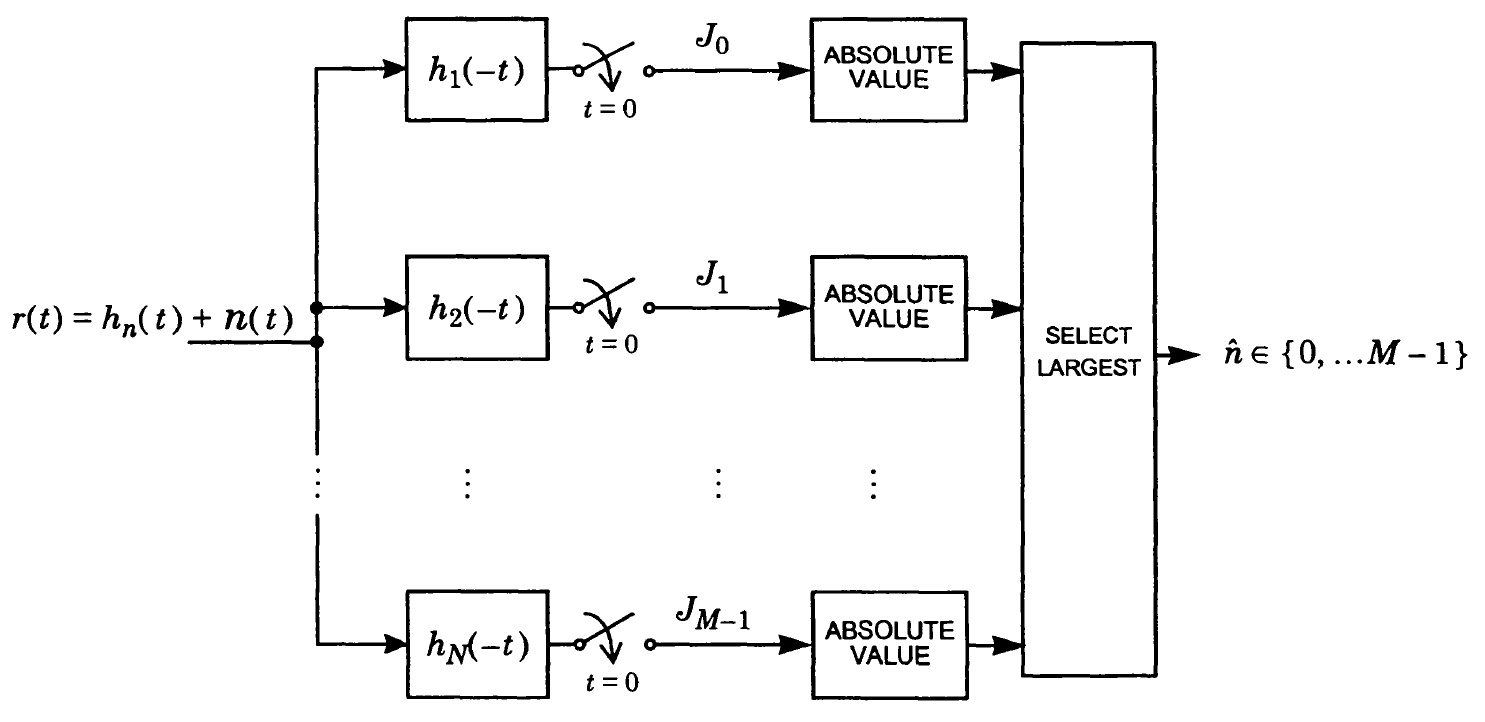
\includegraphics[width=0.75\columnwidth]{figs/adv_26}
		\end{center}
	    \end{figure}
	\end{itemize}	
\end{frame}

\begin{frame}
	\frametitle{Chaveamento de mínimo deslocamento (MSK)}

	\begin{itemize}	   
	    \item Como os sinais de polaridade reversa carregam a mesma informação, o filtro casado no receptor deve comparar o valor absoluto das amostras.
	    \item Esse receptor descarta informações relevantes: baseado no histórico de recepção é possível inferir qual das polaridades seria esperada.
	    \item O uso dessa informação (memória) pode reduzir a probabilidade de erro.
	    \item Os pulsos podem ser reescritos como:
	    \begin{equation*}
		g_i(t) = \sin[2\pi f_c t + \pi bt/(2T) + \phi]w(t)
	    \end{equation*}
	    \item Onde $b \in \{\pm 1 \}$ determina a frequência e $\phi \in \{0, \pi\}$ depende da fase.
	    \item Representação do sinal MSK transmitido:
	    \begin{equation*}
		x(t) = \sum_{k=-\infty}^{\infty} \sin[2\pi f_c t + \pi b_k t/(2T) + \phi_k]w(t-kT)
	    \end{equation*}

	\end{itemize}	
\end{frame}

\begin{frame}
	\frametitle{Chaveamento de mínimo deslocamento (MSK)}

	\begin{itemize}	   
	    \item Para manter a continuidade da fase é necessário que:
	    \begin{equation*}
		\phi_k = \phi_{k-1} + (b_{k-1} - b_k)\pi k/2 \; \mod 2\pi
	    \end{equation*}
	    \item Esta expressão mostra a dependência explícita da fase sobre os dados.
	    \item O desempenho do filtro casado para o MSK binário é semelhante ao do FSK binário.
	    \item É possível reduzir o erro e a banda ao se utilizar informação sobre a memória, levando o desempenho do MSK a ficar equivalente ao do PSK.
	    \item O MSK também pode ser interpretado como sinais PAM de banda passante cuja componente em quadratura é atrasada de meio símbolo com relação à componente em fase.
	    \item Tais sinais são chamados de \textit{offset keyed}: OQAM (OK-QAM) ou OPSK (OK-PSK).
	\end{itemize}	 
\end{frame}

\begin{frame}
	\frametitle{Detecção do CPM}

	\begin{itemize}	   
	    \item Exemplo de diagrama de fase para o MSK:
	    \begin{figure}[t]	
		\begin{center}
		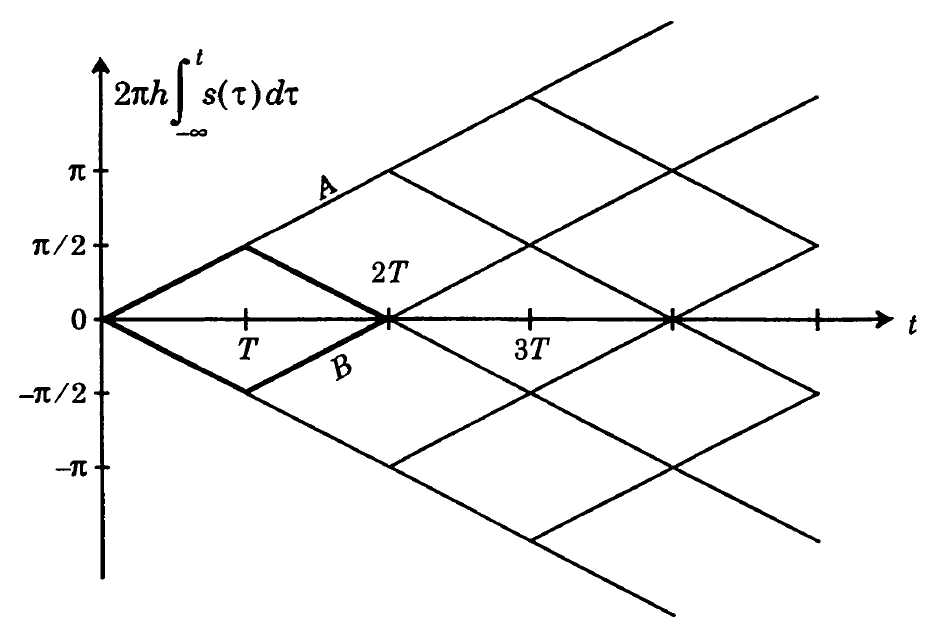
\includegraphics[width=0.65\columnwidth]{figs/adv_27}
		\end{center}
	    \end{figure}
	    \item Algoritmo de Viterbi pode ser empregado na detecção.
	\end{itemize}	 
\end{frame}

\begin{frame}
	\frametitle{Codificação diferencial}

	\begin{itemize}	   
	    \item Várias constelações possuem invariância rotacional para alguns ângulos de rotação.
	    \item Se a constelação for rotacionada de tal ângulo, não há como distinguí-la de uma constelação válida.
	    \item Codificação diferencial evita esses problemas: a informação é codificada pela mudança na posição da constelação, e não pela posição absoluta.
	    \item Aplicação em cenários com desvanecimento rápido.
	    \item Considerando símbolos $a_k = e^{j\phi_k}$, modulação PSK diferencial (DPSK):
	    \begin{equation*}
		   \phi_k = \phi_{k-1} + \Delta_k
	    \end{equation*}
	    \item Informação contida na diferença de fase $\Delta_k$ e não na fase absoluta $\phi_k$.
	\end{itemize}	 

\end{frame}

\begin{frame}
	\frametitle{Codificação diferencial}

	\begin{itemize}	   
	    \item Técnicas de detecção do DPSK: coerente ou diferencial.
	    \item Detecção coerente:
	    \begin{itemize}
	      \item Procura aprender e rastrear a fase absoluta dos sinais recebidos.
	      \item Apropriada quanto a codificação diferencial é utilizada somente para mitigar o efeito da invariância rotacional.
	    \end{itemize}
	    \item Detecção diferencial:
	    \begin{itemize}
	      \item Se baseia somente na diferença de fase entre um símbolo e outro.
	      \item Evita ter que rastrear a fase em ambiente com desvanecimento rápido
	      \item Penalidade de aumento do ruído de aproximadamente 3 dB.
	    \end{itemize}

	    \begin{figure}[t]	
		\begin{center}
		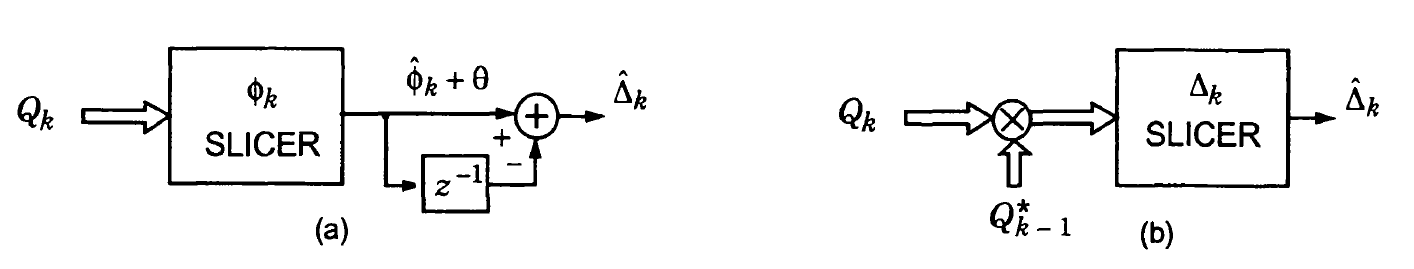
\includegraphics[width=0.8\columnwidth]{figs/adv_28}
		\end{center}
	    \end{figure}
	\end{itemize}	 
\end{frame}

\section{Largura de banda e dimensionalidade do sinal}

\begin{frame}
	\frametitle{Teorema de Landau-Pollak}

	\begin{itemize}	   
	    \item Nenhum sinal pode ser limitado simultaneamente no tempo e na banda.
	    \item No entanto, é possível que sinais limitados em banda sejam \textit{aproximadamente} limitados no tempo. 
	    \item De forma análoga, sinais limitados no tempo podem ser \textit{aproximadamente} limitados na frequência. 
	    \item Seja $f(t)$ causal, limitada a uma banda $W$ Hz e com energia finita $\mathcal{E}_f$.
	    \item Essa função não chegará precisamente a zero em um tempo $t_0$, mas devido à energia finita decairá gradualmente a zero.
 	    \item Seja $\epsilon(t_0)$ a fração da energia de $f(t)$ fora do intervalo $[0,t_0]$, então:
 	    \begin{equation*}
		\int_0^{t_0} |f(t)|^2 dt = \mathcal{E}_f (1-\epsilon(t_0))
 	    \end{equation*}
	    \item É possível portanto definir um intervalo de tempo dentro do qual somente uma fração da energia do sinal está fora do intervalo.
	\end{itemize}	 
\end{frame}

\begin{frame}
	\frametitle{Teorema de Landau-Pollak}

	\begin{block}{Teorema}
	    Existe um conjunto ortonormal de $2Wt_0+1$ formas de onda $\phi_i(t)$, tal que para qualquer forma de onda de energia finita $f(t)$ com energia $\mathcal{E}_f$, limitada em banda a $|f| \leq W$, para qualquer constante $0 < \epsilon < 1$ e para qualquer $t_0$ suficientemente grande e que satisfaça $\int_0^{t_0} |f(t)|^2 dt > \mathcal{E}_f (1-\epsilon(t_0))$, existe também um conjunto de $2Wt_0+1$ coeficientes $f_i$ que satisfaz:
	    \begin{equation*}
		\int_{-\infty}^{\infty} \left| f(t) - \sum_{i=0}^{2Wt_0} f_i \phi_i(t) \right|^2 dt < 12\mathcal{E}_f \epsilon
	    \end{equation*}
	\end{block}
\end{frame}


\begin{frame}
	\frametitle{Teorema de Landau-Pollak}

	\begin{itemize}	   
	    \item O espaço de sinal de sinais de energia finita possui infinitas dimensões.
	    \item No entanto, sinais de banda limitada a $W$ Hz e aproximadamente limitados no tempo em $[0,t_0]$, possuem aproximadamente um número finito de dimensões: $2Wt_0+1$ (Teorema de Landau-Poloak).
	    \item Neste caso somente uma pequena fração da energia do sinal está fora do subespaço de dimensão $2Wt_0+1$.
	    \item À medida em que $t_0$ aumenta, essa fração de energia se reduz.
	\end{itemize}	 
\end{frame}


\begin{frame}
	\frametitle{Relação com o critério generalizado de Nyquist}

	\begin{itemize}
	    \item No critério generalizado de Nyquist não foi feita nenhuma tentativa de limitar os pulsos no tempo.
	    \item No entanto, pode-se demonstrar que o teorema de Landau-Pollak e o critério generalizado de Nyquist são consistentes entre si.
	    \item Considere um sinal ortogonal consistindo de $L$ intervalos de sinalização.
	    \item Em geral, tal sinal é aproximadamente limitado ao intervalo $[0,LT]$.
	    \item A partir do teorema de Landau-Pollak temos que:
	    \begin{equation*}
		2WLT + 1 \geq NL \quad \Longrightarrow \quad W \geq \frac{NL-1}{2LT} \quad \underset{\scriptscriptstyle L\rightarrow \infty}{\Longrightarrow} \quad W \geq N/(2T)
	    \end{equation*}
	    \item Resultado consistente com o critério generalizado de Nyquist.
	\end{itemize}
\end{frame}

\section{Capacidade e modulação}

\begin{frame}
	\frametitle{Capacidade e modulação}

	\begin{itemize}
	    \item Métricas para comparação entre esquemas de modulação:
	    \begin{itemize}
		\item Potência média de transmissão, potência de pico e imunidade ao ruído.
		\item Probabilidade de erro de símbolo (SER), bit (BER) e bloco (BLER).
		\item Eficiência espectral.
		\item Ganho de codificação: redução no nível de potência para atingir uma certa probabilidade de erro (através de técnicas de codificação de canal).
		\item Custo de implementação.
	    \end{itemize}\vspace{0.3cm}
	    \item Considerações para as comparações:
	    \begin{itemize}
		\item Canal ideal com banda $W$ e ruído aditivo Gaussiano branco com DEP $N_0/2$.
		\item Restrição de potência média de transmissão $P$, sem restrição de pico.
		\item SER reflete adequadamente o desempenho do sistema. Limitante da união pode ser usado para obter a BER.
	    \end{itemize}
	\end{itemize}
\end{frame}


\begin{frame}
	\frametitle{Probabilidade de erro do PAM}

	\begin{itemize}
	    \item Expressão da SER como função dos parâmetros relevantes:
	    \begin{equation*}
		P_e \approx K \cdot Q\left(\frac{d_{\min}}{2\sigma} \right) \approx K \cdot Q\left(\sqrt{2WT \cdot \eta_A \cdot \text{SNR}} \right)
	    \end{equation*}
	    \item Considerando $K$ como o número médio de vizinhos com distância mínima $d_{\min}$, $\sigma^2 = N_0/2$, banda $W$, energia média do sinal $\mathcal{E}$, intervalo de símbolos $T$, $P=E/T$, $\text{SNR} = P/(N_0 W)$ e $\eta_A = d_{\min}^2 / (4\mathcal{E}_a)$
	    \item O valor de $\eta_A$ pode ser calculado para diferentes esquemas de modulação.
	    \item Expressão da eficiência espectral:
	    \begin{equation*}
		\nu = \frac{\log_2 M}{WT}
	    \end{equation*}	    
	\end{itemize}
\end{frame}

\begin{frame}
	\frametitle{Probabilidade de erro do PAM}

	\begin{itemize}
	    \item Cálculo da probabilidade de erro considerando a máxima taxa possível pelo critério de Nyquist.
	    \item Para banda base temos $1/T = 2W$ e para banda passante temos $1/T = W$.
	    \item Expressão geral para PAM em banda base, banda passante e constelações QAM quadradas:
	    \begin{equation*}
		P_e \approx K \cdot Q \left(\sqrt{3\cdot \frac{\text{SNR}}{2^{\nu}-1}} \right)
	    \end{equation*}
	    \item SNR normalizada pela taxa:
	    \begin{equation*}
		\text{SNR}_{\text{norm}} = \frac{\text{SNR}}{2^{\nu}-1}
	    \end{equation*}

	\end{itemize}
\end{frame}

\begin{frame}
	\frametitle{Capacidade do canal Gaussiano ideal}

	\begin{itemize}
	    \item Capacidade:
	    \begin{align*}
		C_T &= WT \cdot \log_2(1+\text{SNR}) \\
		C &= C_T/T = W \cdot \log_2(1+\text{SNR})
	    \end{align*}
	    \begin{figure}[t]	
		\begin{center}
		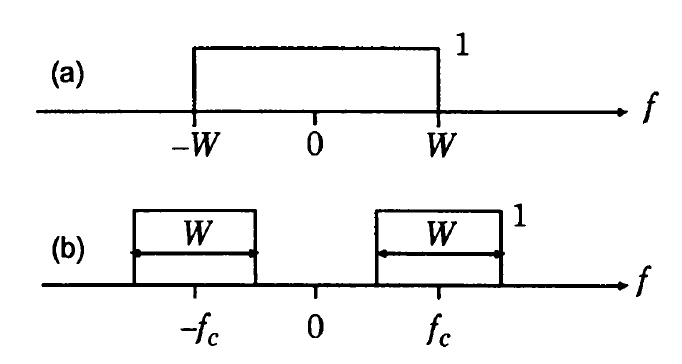
\includegraphics[width=0.55\columnwidth]{figs/adv_29}
		\end{center}
	    \end{figure}
	\end{itemize}
\end{frame}

\begin{frame}
	\frametitle{Capacidade do canal Gaussiano ideal}

	\begin{itemize}
	    \item Diferença entre SNR e seu valor normalizado: $\Delta \text{SNR}_{\text{dB}} = \text{SNR}_{\text{dB}} - \text{SNR}_{\text{norm,dB}}$
	    \begin{figure}[t]	
		\begin{center}
		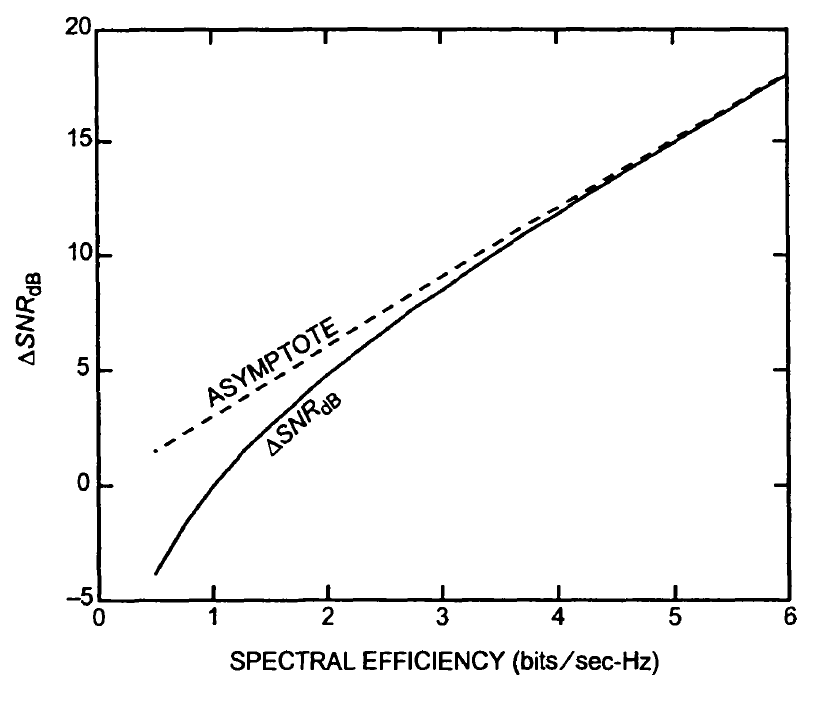
\includegraphics[width=0.6\columnwidth]{figs/adv_30}
		\end{center}
	    \end{figure}
	\end{itemize}
\end{frame}

